\documentclass[
11pt, % The default document font size, options: 10pt, 11pt, 12pt
%oneside, % Two side (alternating margins) for binding by default, uncomment to switch to one side
english, % ngerman for German
singlespacing, % Single line spacing, alternatives: onehalfspacing or doublespacing
%draft, % Uncomment to enable draft mode (no pictures, no links, overfull hboxes indicated)
%nolistspacing, % If the document is onehalfspacing or doublespacing, uncomment this to set spacing in lists to single
%liststotoc, % Uncomment to add the list of figures/tables/etc to the table of contents
%toctotoc, % Uncomment to add the main table of contents to the table of contents
parskip, % Uncomment to add space between paragraphs
%nohyperref, % Uncomment to not load the hyperref package
headsepline, % Uncomment to get a line under the header
chapterinoneline, % Uncomment to place the chapter title next to the number on one line
%consistentlayout, % Uncomment to change the layout of the declaration, abstract and acknowledgements pages to match the default layout
]{MastersDoctoralThesis} % The class file specifying the document structure
\usepackage{url}
\usepackage[utf8]{inputenc} % Required for inputting international characters
\usepackage[T1]{fontenc} % Output font encoding for international characters
\usepackage{lipsum}
\usepackage{mathpazo} % Use the Palatino font by default
\usepackage{fltrace}
\usepackage{float}
\usepackage{hyperref}
\usepackage{tcolorbox}
\usepackage{forest}
\usepackage{rotating}
\usepackage[font=scriptsize]{caption}
\usepackage[colorinlistoftodos,textwidth=30mm,textsize=tiny]{todonotes}
\usepackage[style=authoryear,maxbibnames=9,maxcitenames=2,uniquelist=false,backend=biber]{biblatex} % Use the bibtex backend with the authoryear citation style (which resembles APA)

\usepackage[autostyle=true]{csquotes} % Required to generate language-dependent quotes in the bibliography
\usepackage[acronym, toc]{glossaries}
\usepackage{fontawesome}
\makeglossaries
\loadglsentries{Pages/Abbreviations.tex}
\let\cleardoublepage=\clearpage

%----------------------------------------------------------------------------------------
%  code listings
%----------------------------------------------------------------------------------------
\usepackage{listings}
\usepackage{etoolbox}
\usepackage{color}

\definecolor{base0}{RGB}{131,148,150}
\definecolor{base01}{RGB}{88,110,117}
\definecolor{base2}{RGB}{238,232,213}
\definecolor{sgreen}{RGB}{133,153,0}
\definecolor{sblue}{RGB}{38,138,210}
\definecolor{scyan}{RGB}{42,161,151}
\definecolor{smagenta}{RGB}{211,54,130}
\definecolor{mygray}{gray}{0.98}


\newcommand\digitstyle{\color{smagenta}}
\newcommand\symbolstyle{\color{base01}}
\makeatletter
\newcommand{\ProcessDigit}[1]
{%
  \ifnum\lst@mode=\lst@Pmode\relax%
   {\digitstyle #1}%
  \else
    #1%
  \fi
}
\makeatother


\lstdefinestyle{solarizedcsharp} {
  language=[Sharp]C,
  frame=lr,
  breaklines=true,
  tabsize=2,
  numbers=left,
  numbersep=5pt,
  firstnumber=auto,
  numberstyle=\tiny\ttfamily\color{base0},
  rulecolor=\color{base2},
  backgroundcolor=\color{mygray},
  basicstyle=\scriptsize\ttfamily,
  commentstyle=\color{base01},
  morecomment=[s][\color{base01}]{/*+}{*/},
  morecomment=[s][\color{base01}]{/*-}{*/},
  morekeywords={  abstract, event, new, struct,
                as, explicit, null, switch,
                base, extern, object, this,
                bool, false, operator, throw,
                break, finally, out, true,
                byte, fixed, override, try,
                case, float, params, typeof,
                catch, for, private, uint,
                char, foreach, protected, ulong,
                checked, goto, public, unchecked,
                class, if, readonly, unsafe,
                const, implicit, ref, ushort,
                continue, in, return, using,
                decimal, int, sbyte, virtual,
                default, interface, sealed, volatile,
                delegate, internal, short, void,
                do, is, sizeof, while,
                double, lock, stackalloc,
                else, long, static,
                enum, namespace, string, var},
  keywordstyle=\bfseries\color{sgreen},
  showstringspaces=false,
  stringstyle=\color{scyan},
  identifierstyle=\color{sblue},
  extendedchars=true,
  captionpos=b,
}

\lstset{style=solarizedcsharp}


%----------------------------------------------------------------------------------------
%	RANDOM COMMANDS USED IN THE THESIS
%----------------------------------------------------------------------------------------
\newcommand{\fullref}[1]{chapter \ref{#1} \nameref{#1}}
\newcommand{\code}[1]{\textcolor{sblue}{\textit{\citetitle{#1}}}}
\newcommand{\citecode}[1]{\textcolor{sblue}{\citetitle{#1} \parencite{#1}}}
\newcommand{\mycolorbox}[2]{\begin{tcolorbox}[boxrule=0.1pt, colback=mygray, title={#2} ,colbacktitle=gray]
  \textit{#1}
\end{tcolorbox}}

%----------------------------------------------------------------------------------------
%	FONT ICON COMMANDS
%----------------------------------------------------------------------------------------
\newcommand{\converges}{\faPlus\faPlus}
\newcommand{\diverges}{\faMinus}
\newcommand{\supports}{\faPlus}

%----------------------------------------------------------------------------------------
%	MARGIN SETTINGS
%----------------------------------------------------------------------------------------
\geometry{
	paper=a4paper, % Change to letterpaper for US letter
	inner=2.5cm, % Inner margin
	outer=3.8cm, % Outer margin
	bindingoffset=.5cm, % Binding offset
	top=1.5cm, % Top margin
	bottom=1.5cm, % Bottom margin
	%showframe, % Uncomment to show how the type block is set on the page
}

%----------------------------------------------------------------------------------------
%	THESIS INFORMATION
%----------------------------------------------------------------------------------------

\NewDocumentCommand{\promo}{m}{\newcommand{\promotor}{#1}}
\NewDocumentCommand{\coproone}{m}{\newcommand{\firstco}{#1}}
\NewDocumentCommand{\coprotwo}{m}{\newcommand{\secondco}{#1}}

\thesistitle{On the convergence of the philosophy of Clean Architecture with the Normalized Systems Theorems} % \ttitle
\subject{A Design Science approach of modularity,\\ stability and evolvability of a C\#
software artifact.} % \subjectname

\promo{Prof. Dr. Ing. Hans Mulder}
\coproone{Dr. ir. Geert Haerens}
\coprotwo{Frans Verstreken, MSc}
\degree{Master of Enterprise IT Architecture}
\author{Gerco Koks}

\keywords{} % Keywords for your thesis, this is not currently used anywhere in the template, print it elsewhere with \keywordnames
\university{Antwerp Management School}
\department{\href{http://department.university.com}{Department or School Name}}
\group{\href{http://researchgroup.university.com}{Research Group Name}}
\faculty{Master of Enterprise IT Architecture}

\AtBeginDocument{
\hypersetup{pdftitle=\ttitle} % Set the PDF's title to your title
\hypersetup{pdfauthor=\authorname} % Set the PDF's author to your name
\hypersetup{pdfkeywords=\keywordnames} % Set the PDF's keywords to your keywords
\hypersetup{citecolor=., linkcolor=., urlcolor=.}
}
\pdfinfo{
	/title=\ttitle
}

%----------------------------------------------------------------------------------------
%	Bibliography
%----------------------------------------------------------------------------------------
\setcounter{biburllcpenalty}{7000}
\setcounter{biburlucpenalty}{8000}
\addbibresource{bibliography.bib} % The filename of the bibliography

%----------------------------------------------------------------------------------------
%	Enabling a treeview used in the appendix
%----------------------------------------------------------------------------------------
\definecolor{folderbg}{RGB}{124,166,198}
\definecolor{folderborder}{RGB}{110,144,169}

\def\Size{4pt}
\tikzset{
      folder/.pic={
        \filldraw[draw=folderborder,top color=folderbg!50,bottom color=folderbg]
          (-1.05*\Size,0.2\Size+5pt) rectangle ++(.75*\Size,-0.2\Size-5pt);  
        \filldraw[draw=folderborder,top color=folderbg!50,bottom color=folderbg]
          (-1.15*\Size,-\Size) rectangle (1.15*\Size,\Size);
      }
    }

\begin{document}
\frontmatter % Use roman page numbering style (i, ii, iii, iv) for the pre-content pages

\pagestyle{plain}

%----------------------------------------------------------------------------------------
%	PAGES
%----------------------------------------------------------------------------------------
\begin{titlepage}
    \begin{center}
    
    \vspace*{.06\textheight}
    {\scshape\LARGE \univname\par}\vspace{1.5cm} % University name
    
    {\huge \bfseries \ttitle\par}\vspace{0.4cm} % Thesis title
    {\emph{\large \subjectname}}\vspace{2.4cm}
     
    \begin{minipage}[t]{0.4\textwidth}
    \begin{flushleft} \large
    \emph{Author:}\\
    \authorname % Author name - remove the \href bracket to remove the link
    \end{flushleft}
    \end{minipage}
    \begin{minipage}[t]{0.4\textwidth}
    \begin{flushright} \large
    \emph{Promotor:} \\
    \promotor\vspace{0.2cm} \\
    \emph{Co-Promotors:} \\
    \firstco \\
    \secondco \\
    \end{flushright}
    \end{minipage}\\[3cm]
     
    \vfill
    
    \large \textit{A thesis submitted in fulfillment of the requirements\\ for the degree of \degreename}\\[0.3cm] % University requirement text
     
    \vfill
    
    {\large \today}\\[4cm] % Date
    %\includegraphics{Logo} % University/department logo - uncomment to place it
     
    \vfill
    \end{center}
    \end{titlepage}
\begin{declaration}
\addchaptertocentry{\authorshipname} % Add the declaration to the table of contents
\noindent I, \authorname, declare that this thesis titled, \enquote{\ttitle} and the work presented in it are my own. I confirm that:

\begin{itemize} 
\item This work was done wholly or mainly while in candidature for a research degree at this University.
\item Where any part of this thesis has previously been submitted for a degree or any other qualification at this University or any other institution, this has been clearly stated.
\item Where I have consulted the published work of others, this is always clearly attributed.
\item Where I have quoted from the work of others, the source is always given. With the exception of such quotations, this thesis is entirely my own work.
\item I have acknowledged all main sources of help.
\item Where the thesis is based on work done by myself jointly with others, I have made clear exactly what was done by others and what I have contributed myself.\\
\end{itemize}
 
\noindent Signed:\\
\rule[0.5em]{25em}{0.5pt} % This prints a line for the signature
 
\noindent Date:\\
\rule[0.5em]{25em}{0.5pt} % This prints a line to write the date
\end{declaration}

\cleardoublepage
\vspace*{0.2\textheight}

\noindent\enquote{\itshape I have not failed. Instead, I have 10.000 ways that won't work.}\bigbreak

\hfill Thomas Edison

\noindent\enquote{\itshape Success is not final, failure is not fatal: it is the courage to continue that counts.}\bigbreak

\hfill Winston Churchill

\noindent\enquote{\itshape In all chaos there is a cosmos, in all disorder a secret order.}\bigbreak

\hfill Carl Jung
\begin{abstract}
\addchaptertocentry{\abstractname}
\end{abstract}
\begin{acknowledgements}
\addchaptertocentry{\acknowledgementname} % Add the acknowledgments to the table of contents
The acknowledgments and the people to thank go here, don't forget to include your project advisor\ldots
\end{acknowledgements}
\tableofcontents % Prints the main table of contents
\listoffigures % Prints the list of figures
\listoftables % Prints the list of tables
\printglossary[title=List of Abbreviations, toctitle=List of Abbreviations, type=\acronymtype, nonumberlist]
%\newacronym{ns}{NS}{Normalized Systems}
\newacronym{ca}{CA}{Clean Architecture}
\newacronym{oop}{OOP}{Object-Oriented Programming}
\newacronym{srp}{SRP}{Single Responsibility Principle}
\newacronym{ocp}{OCP}{Open/Closed Principle}
\newacronym{lsp}{LSP}{Liskov Substitution Principle}
\newacronym{isp}{ISP}{Interface Segregation Principle}
\newacronym{dip}{DIP}{Dependency Inversion Principle}
\newacronym{avt}{AvT}{Action Version Transparency}
\newacronym{dvt}{DvT}{Data Version Transparency}
\newacronym{soc}{SoC}{Separation Of Concerns}
\newacronym{sos}{SoS}{Separation of State}
\newacronym{solid}{SOLID}{\acrlong*{srp}, \acrlong*{ocp}, \acrlong*{lsp}, \acrlong*{isp}, \acrlong*{dip}}
\newacronym{bibo}{BIBO}{Bounded Input Bounded Output}
\newacronym{crud}{CRUD}{Creat, Read, Update, Delete}
\newacronym{erd}{ERD}{Entity Relation Diagram}
\newacronym{dll}{DLL}{Dynamic Link Library}
\newacronym{apa}{APA}{American Psychological Association}
\newacronym{vscode}{VSCode}{Visual Studio Code}
\newacronym{mdd}{MDD}{Model Driven Development}
\newacronym{rep}{REP}{The Resuse/Release Equivalence Principle}
\newacronym{ccp}{CCP}{The Common Closure Principle}
\newacronym{crp}{CRP}{The Common Reuse Principle}

\printglossary[title=Abbreviations, toctitle=Abbreviations, type=\acronymtype, nonumberlist]
\dedicatory{For/Dedicated to/To my\ldots} 
 
%----------------------------------------------------------------------------------------
%	THESIS CONTENT - CHAPTERS
%----------------------------------------------------------------------------------------
\mainmatter % Begin numeric (1,2,3) page numbering
\pagestyle{thesis} % Return the page headers back to the "thesis" style

\chapter{Introduction} \label{introduction}

\section{Preamble} \label{sec:preamble}
\enquote{\emph{Pantha Rhei}} is, according to \emph{Plato}, one of the famous
philosophical statements first described by the Greek philosopher
\emph{Heraclitus}\footnote{\url{https://plato.stanford.edu/entries/process-philosophy/}}.
His statement unambiguously describes the dynamics of everything that exists. The
\enquote{flux}, or \emph{change} is one of the constants in life. It can also be applied
to contemporary corporate environments where change is continuously introduced at an
ever-increasing pace. These changes lead to an evolution of requirements impacting the
evolvability, stability and quality of software artifacts like Information Systems.

The \enquote{laws of software evolution} \parencite[]{lehman_programs_1980} refers to a
series of laws described by \citeauthor{lehman_programs_1980}. He describes the balance
between the forces driving new requirements on the one hand, and the forces that slow down
progress on the other hand. In other words: changing software leads to deterioration of
stability and evolvability, possibly with a negative effect on the desired quality
of these software systems. 

More than a half of century of software engineering-, and architecture practices show that
the complexity of these software artifacts gradually increases over time. Eventually, this
will render most of the software artifacts obsolete, according to
\citeauthor{lehman_programs_1980} \parencite[]{lehman_programs_1980}.

Over time there have been many attempts to solve the deterioration of Software Artifact,
some of which with scientific backgrounds. Even before the publication of
\citeauthor{lehman_programs_1980} laws of evolution, McIlroy proposed a vision where the
systematic reuse of software building blocks leads to negative programming practices where
software changes eventually lead to a reduction of complexity. Parnas continued with the
principle of information hiding which can be considered to be the foundation of modular
software architectures.

Over the last decades, several programming paradigms had had a significant effect on the
modularity, stability and evolvability of software systems. Procedural programming was one
of the first paradigms to emerge that supported modularity in its constructs. This was
then followed by object-oriented with support for encapsulation and polymorphism.
functional programming. All of which had a significant impact on modern programming
languages like Java and C\#. The constructs of these programming languages significantly
enhanced the capabilities of modular and evolvable software architectures. 

\section{Research Problem: The plethora of proposed design \\ principles}
\label{sec_research_problem}

Design principles, patterns, and theorems are, on top of all, additional measures to
enhance the modularity, stability, and evolvability of software artifacts. This thesis
focuses on two prevalent approaches to researching the hypothesized convergence, namely
\gls{ns} and \gls{ca}. introduced in \ref{sec_into_ca} and \ref{sec_inro_ns}. 

A wide variety of proposed design principles are available for the challenges that occur
in modular and evolvable software architecture. Many great experiences documented
throughout professional and personal blog posts on the internet \parencites{noauthor_dont_nodate,
noauthor_generalization_nodate, noauthor_law_nodate}. Unfortunately, many
experiences have mixed outcomes, some are opinionated, and results are sometimes based on
improper interpretations of the proposed solutions.

Deciding on the best fit for one of the solutions is a recurring and often challenging task
for software architects. A popular and widely accepted solution from software engineering
literature is \gls{ca}. There is a broad supporting community, and many corporate
solutions move toward architectures similar to the \gls{ca}
approach. 

An architecture that derives from science and empirical evidence is \gls{ns}
\parencite{mannaert_normalized_2009,mannaert_normalized_2016}. Deciding between the two
approaches can be a challenging task with little documentation and research. Is it
possible that combining the two approaches can be an method that leads to a highly modular
and evolvable software artifact? Let us start with a small introduction to both
approaches.
\section{Introduction to Clean Architecture} \label{sec_into_ca}

\ca is the accumulation of more than half a century of coding, designing, and
architecting software systems by \citeauthor*[]{robert_c_martin_clean_2018}. He published
his experience in his book \citetitle*[]{robert_c_martin_clean_2018} in
\citeyear[]{robert_c_martin_clean_2018}. In this book, he states that creating a software
artifact requires less skill and knowledge. However, creating stable and evolvable
software artifacts is a skill that requires a lot of knowledge, skill, dedication, and
time.

The book aims for a software architecture that minimizes the human resources required to
build and maintain the information system. Like \ns, it has a
prescribed design of software classes that will lead to a modular architecture with low
coupling and high cohesion \parencite{robert_c_martin_clean_2018}.

\section{Introduction on Normalized Systems} \label{sec:inro_ns}

The Normalized Systems theorems are a scientific approach to creating software systems
based on the laws for software evolvability. These theorems have resulted in a documented
track record of achieving software stability, in a scientific environment. Effectively, it
prevents the accumulation of combinatorial effects on anticipated change drivers. This
prevents the positive feedback loop and prevents the degradation of the software artifact.
Preventing positive feedback loops has a positive effect on the evolvability of software
artifacts.\parencite[]{mannaert_normalized_2009}. 

\citeauthor[]{mannaert_normalized_2009} have formulated the theorem of Normalized Systems
as prescriptive structures (elements) that lead to a modular architecture with low
coupling and high cohesion. The resulting software architecture will be designed to cope
with future change \parencites[]{mannaert_normalized_2009}.
\section{Hypothesis} \label{hypothesis} 

The proposed hypothesis is that both 'Clean Architecture' and 'Normalized Systems' lead
to a modular software architecture with reduced combinatorial effects. Consequently, both
architectural approaches will lead to improved stability and evolvability of the
Information system.

Both architectural approaches formulate their modular structures independent of any
given programming technology \parencite[]{mannaert_normalized_2009,martin_clean_2018}. As
such, improvements in terms of stability and evolvability are equally applicable for the
C\# artifact used in this research, compared to case studies where Java SE has been used.
\parencites[]{oorts_building_2014, de_bruyn_enabling_2018}.

\begin{figure}[!ht]
    \centering
    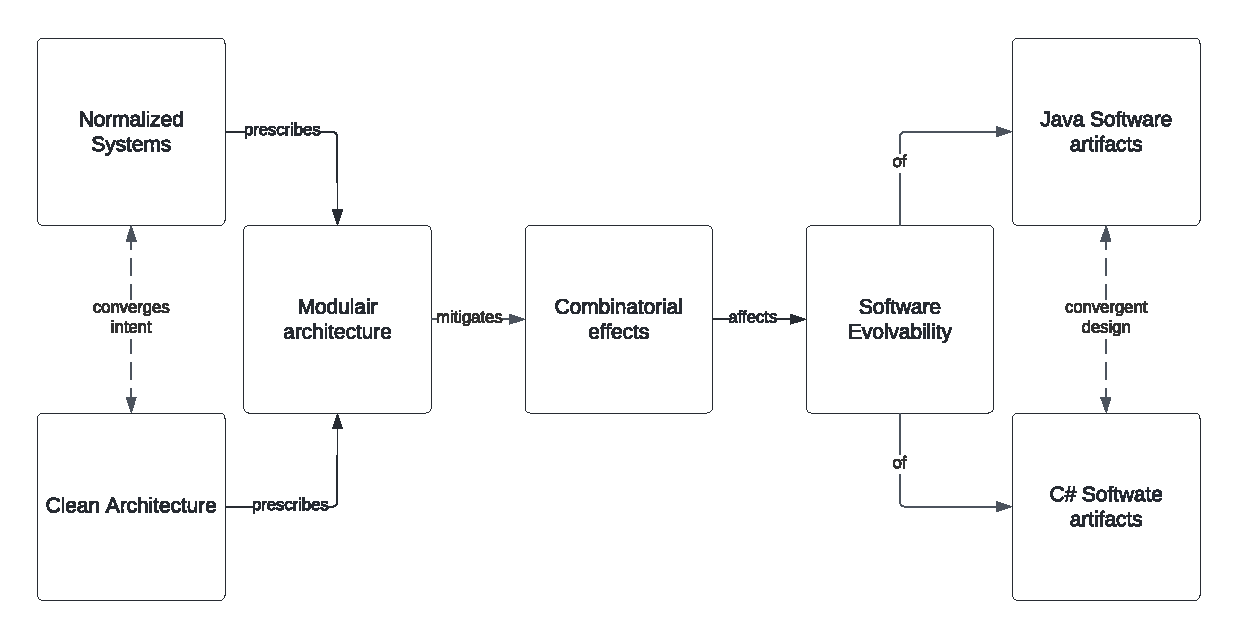
\includegraphics[width=0.9\textwidth]{Figures/hypothesis.pdf}
    \caption[The hypothesis]{The hypothesis}
    \label{fig_hypothesis}
\end{figure}
\section{Research Objectives} \label{sec_research_objectives}

In this Design Science Research, we will shift the focus from Research Questions to
Research Objects. The Object of this research is to determine the degree of convergence of
Clean Architecture, with the Normalized Systems Theory. 

To summarize, we will start with a generic design that is based on the principles and
design characteristics of Clean Architecture. Given this design, we will conduct the
research on two different artifacts, namely a code-generator artifact and a generated
artifact. The reason for the code-generator artifact is to provide strict and meticulous
adherence to the generic design. Each entity should be implemented in exactly the same way.

AFMAKEN



% In this Design Science research, the focus shifts from a research question toward
% research objectives. The following objectives apply to this research.

% \subsection*{Objective 1: The expander artifact}
% A C\# artifact that consists of a source code expander and some helper classes to
% generate the second \emph{expanded} artifact. The artifact supports the harvesting and
% rejuvenation of custom code snippets on the expanded artifact so that regenerations do not
% have a loss of implementations on the expanded artifact. The expander artifact is entirely
% based on the design principles of \gls{ca}.

% Chapter \ref{sec_generator_artifact} entirely describes the expander artifact.

% \subsection*{Objective 2: The expanded artifact}
% This artifact is an entirely working restful API, that is based on ASP.NET and C\#. It has
% essential CRUD support. The artifact has been generated by the \emph{expander} and has
% been enriched with custom code snippets to comply with the initial requirements.
% The expanded artifact is entirely based on the design principles of \gls{ca}.

% Chapter \ref{sec_generator_artifact} entirely describes the expander artifact.


\section{Research questions} \label{research_questions}
The Hypothesis described in \ref{hypothesis} and \ref{conceptualframework} leads us to the
following research question:

\begin{center}
    \enquote*{\textit{To what extent converges the evolvability of a C\# artifact built
    based on the Clean Architecture principles towards a similar artifact that is based on
    Normalized Systems Theorems?}}
\end{center}

The following sub-questions can be formulated that support the research on the main
research question:
\begin{itemize}
    \item How does Clean Architecture contribute to Software Evolvability?
    \item To what extent Is Normalized Systems applicable to a C\# artifact?   
\end{itemize}
\section{Research method} \label{sec_research_method}

This research is a Design Science Method and relies on the Engineering Cycles as described
by \textcite{wieringa_design_2014}. The engineering cycle provides a structured approach
to develop the required artifacts to analyze the design problem (HIER CITE NAAR WIERINGA).

\begin{figure}[H]
    \centering
    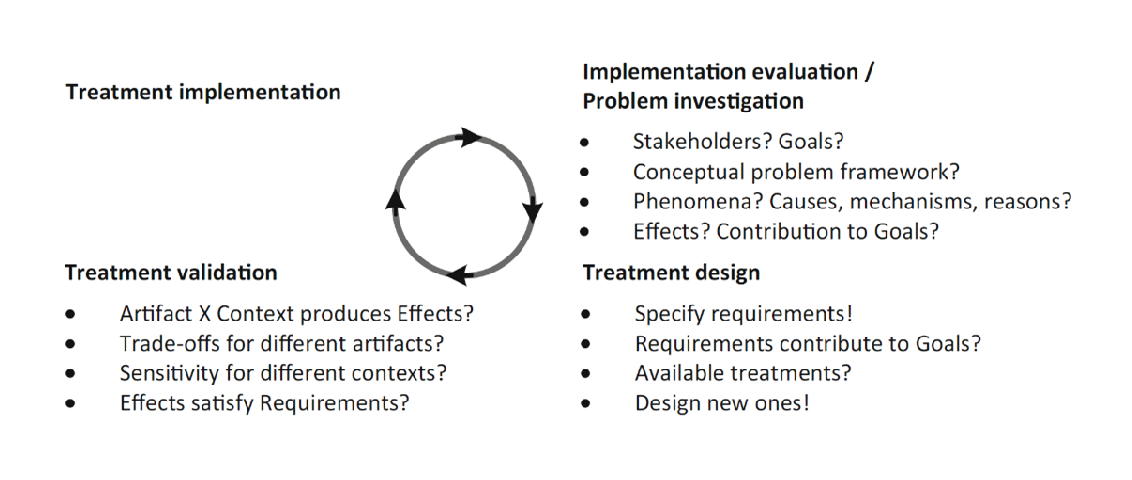
\includegraphics[width=1\textwidth]{Figures/engineering_cycle.pdf}
    \caption[Engineering cycle]{Wieringa's engineering cycle}
    \label{fig_engineering_cycle}
\end{figure}

In the context of this research, the artifacts described in chapters
\ref{sec_generator_artifact} and \ref{sec_generated_artifact} are considered to be
information systems. \citeauthor{hevner_design_nodate} proposed a framework for research
in information systems by introducing the interacting relevance and rigor cycles.

Figure \ref{fig_dsr} depicts a specialized overview of Hevners Design Science Framework.
The rigor cycle is composed of the theories and knowledge from \gls{ns}
and \gls{ca}. This is supplemented by the rigorous knowledge of modularity,
evolvability, and stability of software systems. The Relevance cycle represents the
business needs of the stakeholders. The business needs are described as research
objectives, research questions, and research requirements.

\begin{figure}[H]
    \centering
    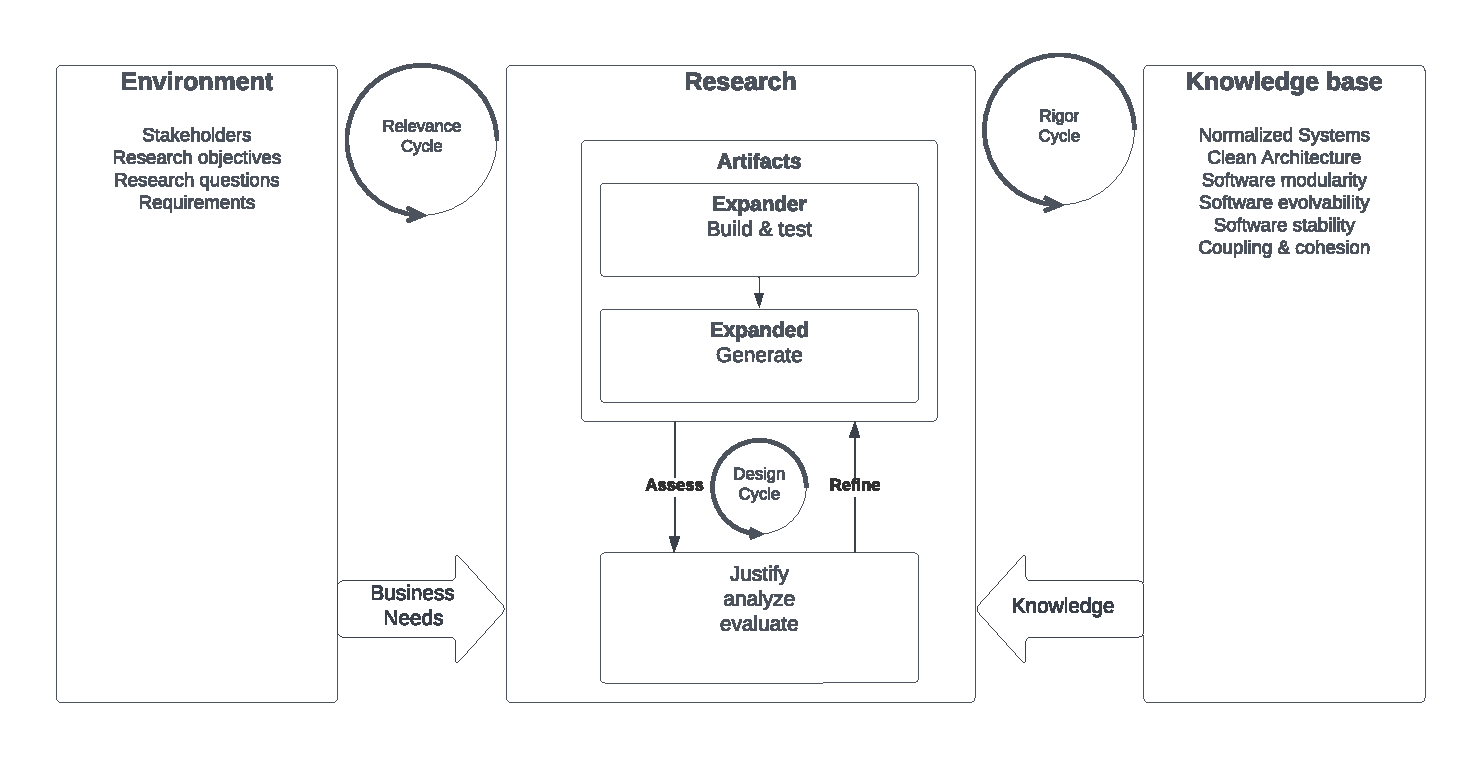
\includegraphics[width=1\textwidth]{Figures/rigor_relevance_cycle.pdf}
    \caption[DSF]{The Design Science Framework for IS Research}
    \label{fig_dsr}
\end{figure}
\chapter{Theoretical background} \label{chap:theoreticalbackground} 

The goal of this thesis is to investigate whether the philosophy of \gls{ca}
aligns with the goals of \gls{ns}. To do so, it is essential to have a
comprehensive understanding of software stability and the key concepts, principles, and
architectures that impact software stability.

This chapter begins by examining the concepts of software stability, evolvability, and
modularity, highlighting their significance in achieving software stability in \gls{ns}.
This is followed by a brief overview of the design theorems and proposed architecture of
\gls{ns}.

The subsequent sections of the thesis explore the fundamental principles that underlie
\gls{ca}, as well as its proposed architecture designs. Finally, the thesis
concludes by discussing which aspects of \gls{ca} align with the principles of
\gls{ns} and contribute to achieving software stability in this approach.

\section{The Theoretical background of Normalized Systems} \label{ns_theory}
\begin{itemize}
    \item Inleiding
\end{itemize}


\subsection{Design Theorems of Normalized Systems} \label{subsec:ns_desing_theorems}


\subsubsection{Separation of Concerns}
\begin{itemize}
    \item Toelichting op SoC
\end{itemize}

\subsubsection{Data version transparancy}
\begin{itemize}
    \item Toelichting op data version transparancy
\end{itemize}

\subsubsection{Action version transparancy}
\begin{itemize}
    \item Toelichting op action version transparancy
\end{itemize}

\subsubsection{Separation of state}
\begin{itemize}
    \item toelichting op Separation of state.
\end{itemize}

\subsection{Construction elements}
\begin{itemize}
    \item Data elements
    \item task elements
    \item connector elements
    \item flow elements
    \item etc\dots
    \item In het hoofdstuk evaluation wordt
    besproken in hoeverre de CA construction elements convergeren met die van NS
\end{itemize}

\section{Towards stable software architectures} \label{sec:on_stability}


\gls{ns} originated in the field of software engineering, aiming to achieve modular and
stable software artifacts. However, the underlying theory of \gls{ns} can be applied to
various other domains, such as Enterprise Engineering, Business Process Modeling, and
document management. This research acknowledges the software engineering background of
gls{ns}. It consistently refers to software and Information Systems when referring to
\enquote*{artifacts}. However, the reader should realize that the concepts and artifacts
are not restricted to software artifacts alone.

In several disciplines stability has been defined as \emph{Bounded Input Bounded Output}
(BIBO). It is the fundamental property of a system when subjected to bounded input
disturbances. BIBO stability ensures that the output of a system will also be bounded,
preventing uncontrolled or unexpected behavior \parencite[270]{mannaert_normalized_2016}. 

A real-world example of the importance of stability is the Tacoma Narrows Bridge in
Washington State, USA. The bridge, depicted in figure \ref*{fig:bridge}, collapsed on
November the 7th, 1940. This was caused due to wind-induced oscillations called
aeroelastic flutter. The wind (Input) induced oscillations in the bridge, causing it to
start swaying back and forth (Output). These oscillations were initially small, but as
they continued, they began to increase in amplitude or magnitude, causing the bridge to
collapse.

\begin{figure}[H]
    \centering
    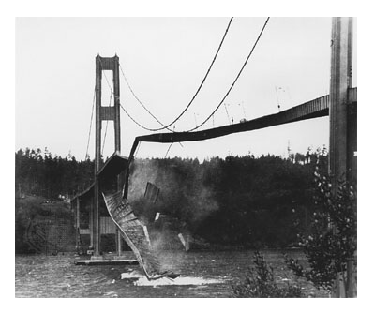
\includegraphics[width=0.6\textwidth]{Figures/bridge.pdf}
    \caption[TNB]{Tacoma Narrows Bridge (Galloping Gertie)}
    \label{fig:bridge}
\end{figure}

Stability can also be used in the context of software engineering. In the context of
\gls{ns}, it is considered a critical property that ensures that the software is not
excessively sensitive to small changes \parencite[270]{mannaert_normalized_2016}. New
functional requirements should only lead to fixed, and an expected amount of changes in
the source code. Conversely, instabilities occur when the total number of modifications
relies on the size of the software artifact. The number of changes will grow over time in
parallel with the growth of the software artifact. These instabilities are referred to as
combinatorial effects \parencite[270]{mannaert_normalized_2016}. when combinatorial effects
are absent, the software artifact can be considered evolvable.
\section{Software evolvability} \label{software_evolvability}

An important aspect of this thesis is to determine the evolvability of software artifacts
with a Clean Architecture design. An evolvable software artifact should not have
instabilities: a bounded amount of additional functional requirements cannot lead to an
unbounded amount of additional (versions of) software primitives \parencite[273]{mannaert_normalized_2009}. 

\subsection{Stability}
<<verwijzing naar positive feedback loops uit de theorie van NS en de effect op
evolueerbaarheid van software.>>

\subsection{Combinatorial effects \& anticipated change drivers.}
<<heeft relatie tot hoofdstuk evaluation en toelichtingen dat software aanpassingen niet
zouden moeten leiden tot een toename in combinatorial effects>>

\subsection{Modularity}
<<toelichten waarop modularity invloed heeft op de evolueerbaarheid van de software>>


\section{Towards evolvable software architectures} \label{sec:on_modules}

There are a couple of aspects concerning evolvable software architectures. One of which is
stability, as described in chapter \ref{sec:on_stability} \nameref{sec:on_stability}.
Another factor that impacts evolvability is the modularity of the architecture. There is a
wide consensus about two fundamental rules when thinking of-, and designing modularity:
\emph{high cohesion} and \emph{low coupling} \autocite[22]{mannaert_normalized_2016}.
These will

Software modules can be defined as self-contained units of code that perform specific
tasks or sets of tasks within a larger system. A software module is designed to operate
independently of other modules, with well-defined interfaces that allow it to communicate
and exchange data with other modules if necessary \autocite[22]{mannaert_normalized_2016}.

A module can be considered a hierarchical and recursive concept. They are independent of
their size (lines of code) or computational magnitude. They can be as small as a function
as part of a class. The class itself can also be considered a module. A group of classes
contained in a Dynamic Link Library (DLL) or Application Programming Interface (API) can
also be considered a module of an even bigger system. 

An important part of the design of a software system is to identify the possible different
modules and their interaction interfaces.

\subsection{Cohesion: The beauty of Software Desing} \label{subsec:on_modularity}

The term cohesion denotes the extent to which the various structural components of a
software system operate cohesively towards a singular and well-defined objective or goal.
Empirical studies in software engineering have extensively demonstrated the significance
of cohesion, linking higher levels of cohesion with reduced defects, enhanced
maintainability, and greater openness to change. Consequently, achieving high cohesion has
been associated with an overall improvement in software quality attributes such as
reliability, maintainability, reusability, and evolvability.

Cohesion facilitates the reduction of complexity and interdependence among the components
of a system, thereby contributing to a more efficient, maintainable, and reliable system.
By organizing components around a shared purpose or function, or by standardizing their
interfaces, data structures, and protocols, cohesion can offer the following benefits:

\begin{itemize}
    \item \textbf{Reduce redundancy and duplication of effort}: \\
    Cohesion ensures that components are arranged around a common purpose or function,
    reducing duplicates or redundant code. This simplifies system comprehension,
    maintenance, and modification.
    \item \textbf{Promoting code reuse:}\\
    Cohesion facilitates code reuse by making it easier to extract and reuse components
    designed for specific functions. This saves time and effort during development and
    enhances overall system quality.
    \item \textbf{Enhance maintainability:}\\
    Cohesion decreases the complexity and interdependence of system components, making it
    easier to identify and rectify bugs or errors in the code. This improves system
    maintainability and reduces the risk of introducing new errors during maintenance.
    \item \textbf{Increase scalability:}\\
    Cohesion improves a system's scalability by enabling it to be extended or modified
    effortlessly to accommodate changing requirements or conditions. By designing
    well-organized and well-defined components, developers can easily add or modify
    functionality as needed without disrupting the rest of the system.  
\end{itemize}

\subsection{Coupling: The beast of Software Desing} \label{subsec:on_coupling}

Coupling is a central concept in software engineering that pertains to the degree of
interdependence among software modules or components. The level of coupling between
modules denotes the strength of their relationship, whereby a high level of coupling
implies a significant degree of interdependence. Conversely, low coupling signifies a
weaker relationship between modules, where modifications in one module are less likely to
impact others.

The negative impacts of excessive coupling on software systems are considerable. High
coupling can render software systems difficult to maintain, modify, or evolve. It can
impede the identification and resolution of errors within a system, leading to prolonged
debugging periods. Additionally, it can cause fragility in the system, where slight
modifications in one module can trigger cascading failures throughout the entire system.
Therefore, it is crucial for software engineers to minimize coupling between modules while
maintaining a cohesive design. By developing systems with low coupling, software engineers
can construct more maintainable, scalable, and adaptable systems that are easier to evolve
over time.

Coupling, in software engineering, can take several forms, including content, common,
control, stamp, and data coupling. Content coupling occurs when one module accesses or
modifies the internal data or logic of another module, leading to high interdependence and
difficulty in isolating errors. Common coupling occurs when several modules access and use
the same global data, increasing their interdependence and reducing modularity. Control
coupling occurs when one module controls the execution flow of another module, making it
difficult to modify or reuse the controlled module. Stamp coupling arises when two modules
share a common data structure, leading to tight coupling and high interdependence.
Finally, data coupling exists when two modules share data, which can lead to coupling
between them.

To avoid the negative impacts of coupling on software systems, software engineers should
aim to minimize the degree of coupling between modules. This can be achieved by designing
cohesive, loosely coupled modules with well-defined interfaces. Loose coupling enables
each module to operate independently, reducing the impact of modifications made to other
modules. By implementing modular design principles, such as high cohesion and low
coupling, software engineers can develop systems that are easier to maintain, test, and
evolve.

In conclusion, coupling is a critical concept in software engineering that can have a
considerable impact on the maintainability, flexibility, and scalability of software
systems. By minimizing coupling between modules, software engineers can develop more
robust, adaptable systems that are easier to modify and evolve. Adopting modular design
principles can also facilitate the development of cohesive, loosely coupled modules that
enable the independent operation and reduce the impact of modifications made to other
modules.
\subsubsection{Cohesion} \label{subsubsec:on_cohesion}

The term cohesion denotes the extent to which the various structural components of a
software system operate cohesively towards a singular and well-defined objective or goal.
Empirical studies in software engineering have extensively demonstrated the significance
of cohesion, linking higher levels of cohesion with reduced defects, enhanced
maintainability, and greater openness to change. Consequently, achieving high cohesion has
been associated with an overall improvement in software quality attributes such as
reliability, maintainability, reusability, and evolvability.

Cohesion facilitates the reduction of complexity and interdependence among the components
of a system, thereby contributing to a more efficient, maintainable, and reliable system.
By organizing components around a shared purpose or function, or by standardizing their
interfaces, data structures, and protocols, cohesion can offer the following benefits:

\begin{itemize}
    \item \textbf{Reduce redundancy and duplication of effort}: \\
    Cohesion ensures that components are arranged around a common purpose or function,
    reducing duplicates or redundant code. This simplifies system comprehension,
    maintenance, and modification.
    \item \textbf{Promoting code reuse:}\\
    Cohesion facilitates code reuse by making it easier to extract and reuse components
    designed for specific functions. This saves time and effort during development and
    enhances overall system quality.
    \item \textbf{Enhance maintainability:}\\
    Cohesion decreases the complexity and interdependence of system components, making it
    easier to identify and rectify bugs or errors in the code. This improves system
    maintainability and reduces the risk of introducing new errors during maintenance.
    \item \textbf{Increase scalability:}\\
    Cohesion improves a system's scalability by enabling it to be extended or modified
    effortlessly to accommodate changing requirements or conditions. By designing
    well-organized and well-defined components, developers can easily add or modify
    functionality as needed without disrupting the rest of the system.  
\end{itemize}


\subsubsection{Coupling} \label{subsec:on_coupling}

Coupling is an important concept in software engineering that pertains to the degree of
interdependence among software modules and components. The level of coupling between
modules denotes the strength of their relationship, whereby a high level of coupling
implies a significant degree of interdependence. Conversely, low coupling signifies a
weaker relationship between modules, where modifications in one module are less likely to
impact others. Although not always possible, the level of coupling between the various
modules of the system should be kept to a bare minimum.

The negative impact of excessive coupling on software systems is considerable. High
coupling can render software systems difficult to maintain, modify, or evolve. It can make
it considerably more difficult to find the root cause of potential bugs. Additionally, it
causes fragility in the system, where slight modifications in one module can trigger
cascading failures throughout the entire system. Therefore, it is crucial for software
engineers to minimize coupling between modules while maintaining a cohesive design. By
developing systems with low coupling, software engineers can construct more maintainable,
scalable, and adaptable systems that are easier to evolve.

Coupling, in software engineering, can take several forms, including content, common,
control, stamp, and data coupling. Content coupling occurs when one module accesses or
modifies the internal data or logic of another module, leading to high interdependence and
difficulty in isolating errors. Common coupling occurs when several modules access and use
the same global data, increasing their interdependence and reducing modularity. Control
coupling occurs when one module controls the execution flow of another module, making it
difficult to modify or reuse the controlled module. Stamp coupling arises when two modules
share a common data structure, leading to tight coupling and high interdependence.
Finally, data coupling exists when two modules share data, which can lead to coupling
between them.

One attempt to lower coupling in the expanded artifact is to prefer stamp coupling over
data coupling through the API interface. This is done by making use of RequestModels and
ViewModels, instead of the actual data element (see example in Listings \ref{SnipModelExamples}).
Depending on the use case only the required data is passed down to the view, or in the
case of a command accepted as an input parameter.

\lstinputlisting[
    caption={The ViewModel \parencite{koks_componentviewmodel_2023} and RequestModel
    \parencite{koks_deletecomponentcommand_2023} of the Entity 'Component'
    \parencite{koks_gc_component_2023}},
    label={SnipModelExamples}]
    {Snippets/ModelExamples.cs}

\subsection{The Design Theorems} \label{subsec:ns_desing_theorems}

\gls{ns} Theorems is a theoretical framework of principles that aims to enhance the
stability of a software artifact. \gls{ns} provides a rigorous mathematical foundation
that offers guidelines for designing and developing software systems. The principles of NS
have gained significant attention in both academic and industrial circles due to their
potential to increase the evolvability and stability of software artifacts while reducing
maintenance costs. The theorems have been scientifically established and proven. In the
following sections, we will focus on the theorems of \gls{ns}. When applicable, we
emphasize some manifestations in one of the artifacts to demonstrate the level of
convergence of \gls{ca}.
\subsubsection{Separation of Concerns}

Since the early years of software engineering, \gls{soc} has been one of the fundamental
software design principles. The concept itself was introduced by
\citeauthor{parnas_criteria_1972} with his introduction of Information Hiding
\parencite{parnas_criteria_1972}. \gls{soc} as a principle has first been mentioned by
\citeauthor{dijkstra_selected_1982}\footnote{\url{https://en.wikipedia.org/wiki/Separation_of_concerns}}
as the crucial principle to design modular software architecture
\parencite[]{dijkstra_selected_1982}. 

\gls{soc} promotes the idea that a program should be divided into distinct sections, each
addressing a separate concern or aspect of a design problem. This allows for a more
organized and maintainable source code. When implemented correctly, a change to one
concern does not affect the others. \gls{soc} should be applied at the level of individual
modules, rather that the level of an entire program.

The \gls{soc} had its effect on later versions of software design principles like SOLID.
It also influenced \gls{ns}, although it has a more strict definition of this principle.
In the book of \citeauthor{mannaert_normalized_2016} it is described as followed: 

\begin{tcolorbox}
    \begin{center}
        \textbf{Theorem I}\\
        \textit{A processing function can only contain a single task to achieve stability.}    
    \end{center}        
\end{tcolorbox}

There are various manifestations of \gls{soc} observable in the artifacts. One of which is
already mentioned in Figure \ref{fig:modulair_components}, where \gls{soc} is applied to
separate the domain logic from the application, infrastructure and presentation logic.

Another example is the separation of handlers as part of the Clean Architecture Expander.
Each of those handlers executes an isolated part of the expanding process. Consider the
\citetitle{koks_expandentitieshandlerinteractor_2023}
\parencite{koks_expandentitieshandlerinteractor_2023} for example. This Handler is solely
responsible for the generation of Data Entities. 

\begin{figure}[H]
    \centering
    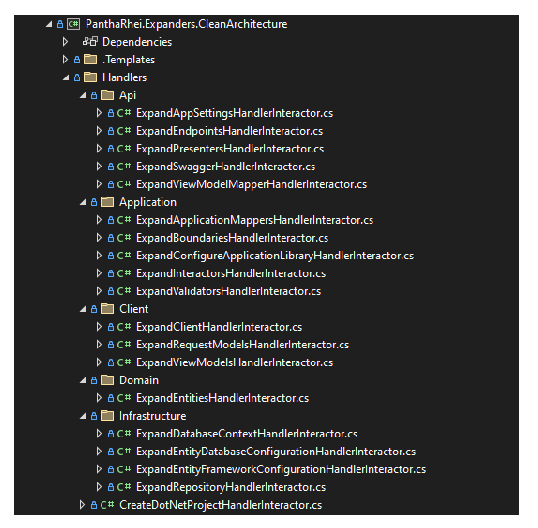
\includegraphics[width=0.8\textwidth]{Figures/expander_handlers.pdf}
    \caption[handlers]{Each of the handlers handles an isolated part of the expanding process.}
    \label{fig:handlers}
\end{figure}
\subsubsection{Data version Transparancy}

\gls{dvt} is the act of encapsulation of data entities for specific tasks at hand. This
results in the fact that data structures can have multiple versions often mentioned as
Data Transfer Objects in modern software engineering projects. In other words, it should
be possible to update the data entity without affecting the processing functions. This
leads to the following description of the theorem \parencite[280]{mannaert_normalized_2016}.

\begin{tcolorbox}
    \begin{center}
        \textbf{Theorem II}\\
        \textit{A data structure that is passed through the interface of a processing function 
        needs to exhibit version transparency in order to achieve stability.}
    \end{center}    
\end{tcolorbox}

\gls{dvt} is widely used in various technological applications. practically every web
service currently known supports some type of versioning. In restful APIs for example, it
is common practice to support versioning over the URI. It is considered a best practice
to encapsulate breaking changes in a new version of the endpoint/service so that the
consumers are not (directly) affected by the change. In modern Object Oriented languages,
gls{dtv} is also supported by the ability to determine the scope of visibility of the
modifiers of the various programming constructs like fields, properties, interfaces and
classes. Also known as information hiding
\parencites{parnas_criteria_1972}[278]{mannaert_normalized_2016}.

The prototype also uses information hiding very strictly. In order to seal implementations
to the intended layers, concrete implementations always have internal visibility, making
them impossible to use. The interfaces on the other hand are publically exposed. The
dependent layers are now restricted to the appointed dependency injection container of the
specific layer. Alternatively, it is also possible to implement a custom implementation of
the specific interface. 

Another example from the prototype is the use of ViewModels for the queries, and
CommandModels for the commands. Depending on the context of the operation, the containing
fields of the Model may differ. A CommandModel for deleting a data entity will only
contain the key of the entity that needs to be deleted. The CommandModel for creating the
same type of entity will probably contain all the required fields of the data entities,
except the key field as this key is often auto-generated by the database or
domain layer of the application.
\subsubsection*{Action version Transparancy}
\gls{avt} is the property of a system to modify existing processing functions without
affecting the existing ones. It should be possible to upgrade a function without affecting
the callers of those functions. This description leads to the following theorem
\parencite[282]{mannaert_normalized_2016}.

\begin{tcolorbox}[boxrule=0.1pt, colback=mygray, title=Theorem III,colbacktitle=gray]
    \textit{A processing function that is called by another processing function, needs to exhibit version transparency in order to achieve stability.}
\end{tcolorbox}

Most of the modern technology environments support some form of \gls{avt}. Polymorphism is
a widely used technique in order to support this theorem. Specifically, parametric
polymorphism \footnote{\url{https://en.wikipedia.org/wiki/Parametric_polymorphism}} allows
for a processing function to have multiple input parameters. There are also quite some
design patterns supporting this theorem. Some random examples are the state pattern
\footnote{\url{https://en.wikipedia.org/wiki/State_pattern}}, facade pattern
\footnote{\url{https://en.wikipedia.org/wiki/Facade_pattern}} and observer pattern
\footnote{\url{https://en.wikipedia.org/wiki/Observer_pattern}}.
\subsubsection{Separation of State}

\gls{sos} is a theorem that is based on the idea that processing functions should not
contain any state information but instead should rely on external data structures to store
state information. By separating state information from processing functions, Normalized
Systems can achieve a higher level of flexibility and adaptability. External data
structures can be updated or replaced without affecting the processing functions
themselves, which greatly reduces the change of unwanted ripple effects. This theorem is
described as followed: \parencite[258]{mannaert_normalized_2016}.

\begin{center}
    \textbf{Theorem IV}\\
    \textit{Calling a processing function within another processing function, needs to exhibit state keeping in order to achieve stability.}
\end{center}

\gls{sos} fits very well in distributed information systems with asynchronous calls. The
expanded artifact is designed in a manner that all external process functions are executed
asynchronously. \todo{snippet toevoegen.}.

A simpler manifestation of the \gls{sos} theorem involves the use of Resources as an
integral part solution
\footnote{url{https://learn.microsoft.com/en-us/dotnet/core/extensions/resources}}. In
addition to enabling the localization of strings, this approach offers the advantage of
centralized management, thereby exhibiting \gls{sos}. For instance, when the functional
requirements evolve, the name of a template in the expander artifact is likely to change.
As the name of the template is used in multiple class instances, a centralized approach to
managing the template name can mitigate the risk of excessive modifications when a name
change is mandated.

Another example. The state of the model (see chapter \ref{sec:artifact_model}) is
currently persisted in an Azure SQL Database.

\lstinputlisting[
    caption={The \citetitle{koks_genericrepository_2023} \parencite{koks_genericrepository_2023}}]
    {Snippets/GenericRepository.cs}

The state of of the expander artifact model as described in \ref{sec:artifact_model} for the expander in the 
voorbeeld met seerders...
voorbeeld met repositories....
\subsection{On the emergence of element} \label{subsec:ns_elements} 

\textbf{Data Element}\\
This is an object that represents a piece of data in the system. Data elements are used to
pass information between processing functions and other objects. In Normalized Systems,
data elements are typically standardized to ensure consistency across the system.

\textbf{Flow Element}\\
This object represents the flow of control through the system. It determines the order in
which processing functions are executed and can be used to handle error conditions or
other exceptional cases.

\textbf{Connector Element}\\
This object is used to connect different parts of the system together. Connectors can be
used to link processing functions, data elements, and other objects, allowing them to work
together seamlessly.

\textbf{Task Element}\\
This is an object that represents a specific task or action in the system. Tasks can be
composed of one or more processing functions and can be used to represent complex
operations within the system.

\section*{The Theoretical background of Clean architecture}

\subsection*{Introduction}

\chapter{Requirements} \label{chap_requirements} 

In this chapter, we will explain that the artifact requirements are composed of two
distinct parts. The research aims to examine the level of convergence between \ca and
\ns. As such, the design and architecture requirements are intentionally, and entirely 
based on the principles and design approach of \ca. A full description of this requirement
can be found in section \ref{sec_artifact_requirements}. In order to analyze the level of
convergence, the artifacts need to comply with the evolvability requirements of the theory
of \ns, described in section \ref{sec_research_requirements} of this chapter.

\section{Research requirements} \label{sec:research_requirements} 

In order to address \nameref{rq1} and \nameref{rq2} we outlined in Chapter
\ref{sec:research_questions}, we need to know what violations in the context of \gls{ns}
can occur in a software artifact. In chapters \ref{sec:ns_theory} we have shown that
\gls{ns} attempts to achieve evolvability by achieving stability. Through the extensive
and consistent use of the \gls{ns} theorems, a modular design emerges that is free of
instabilities. Alternatively, in terms used by the \gls{ns} theorem: the absence of combinatorial
effects. However, as described in section \ref{sec:artifact_requirements}, the artifacts
are designed based on the principles and philosophy of \gls{ca}. The \gls{ns} theorems are
not considered using the design phase of the artifacts. 

To be able to analyze the stability of the artifacts the following functional requirement
specifications are reused \parencite[254-259]{mannaert_normalized_2016}. They are noted
without the mathematical formulas that are present in cited sources.


\mycolorbox{An information system needs to be able to represent instances of data
entities. A data entity consists of a number of data fields. Such a field may be a basic
data field representing a value of a reference to another data entity.}
{Research Requirement 1}

\mycolorbox{An information system needs to be able to execute processing actions on
instances of data entities. A processing action consists of a number of consecutive
processing tasks. Such a task may be a basic task, i.e., a unit of processing that can
change independently, or an invocation of another processing action.}
{Research Requirement 2}

\mycolorbox{An information system needs to be able to input or output values of instances of data entities through connectors.}
{Research Requirement 3}

\mycolorbox{An existing information system representing a set of data entities, needs
to be able to represent: 
\begin{itemize}
    \item a new version of a data entity Dm that corresponds to including an additional
    data field
    \item an additional data entity 
\end{itemize}}
{Research Requirement 4}

\mycolorbox{An existing information system providing a set of processing actions,
needs to be able to provide:
\begin{itemize}
    \item a new version of a processing task, whose use may be mandatory
    \item a new version of a processing action, whose use may be mandatory
    \item an additional processing task
    \item an additional processing action
\end{itemize}}
{Research Requirement 5}
\section{Artifact requirements} \label{sec:artifact_requirements}

The artifacts adhere to the design philosophy of \gls{ca}, described in chapter
\ref{sec:ca_theory}, as much as possible. In order to do so the following
requirements are to be applied.

\subsection{Artifact components}
In \fullref{subsec:layers} we describe that in a typical application, one of the goals of
\gls{ca} is to separate the domain logic from Impl details like (user) interface
or storage mechanisms. Therefore, the artifact must follow the layered architecture of
\gls{ca} (see figure \ref{fig:modulair_components})

In the case of the \nameref{sec:generator_artifact} there are two separate infrastructure
layers. The first one has a dependency on
EntityFrameworkCore\footnote{\url{https://learn.microsoft.com/en-us/ef/core/}} technology
for data persistence in an Azure SQL database. The other one handles persistence by
serialization of data on a windows machine.

\subsection{Flow of control}
One of the \gls{solid} design principles is the \acrfull{dip}. This principle affects the.
As described in \fullref{sebsec:dependency_rule}, this affects the flow of control of the
artifacts components. To achieve the evolvability of each of the components, the flow of
control must adhere to the following statement. This is also depicted in Figure
\ref{fig:modulair_components}.

The component dependencies must point only inward, toward higher-level policies. To make
it more strict, the Presentation and infrastructure layers only depend on the Application
layer The Application layer only depends on the  Domain Layer.

\subsection{Adherence to Design principles}
In \fullref{subsec:design_principles} we describe what needs to be done to adhere to the
\gls{solid} design principles. Each design pattern that is applied to the architecture of
artifacts adheres at least to one of the \gls{solid} principles.

\subsection{Screaming Architecture}
The essence of Screaming Architecture is to design a system where the structure and
purpose of each component and layer are immediately apparent to anyone looking at it. This
is achieved through clear and consistent naming conventions of the classes, namespaces and,
components.

In the literature of \gls{ca}, there is no mention of rules or recommendations for naming
conventions. The most commonly practiced naming convention of nouns (for data entities)
and verbs (for actions) will be used. This is also advocated by the literature of \gls{ns}
\parencite[357]{mannaert_normalized_2016}.

Table \ref{table:component_naming_convention} lists the required naming convention for the
different layers, whereas table \ref{table:element_naming_convention} lists the naming
convention of the recurring elements. For more information about these elements see
\ref{subsec:design_elements}.

\begin{table}[h]
    \small
    \begin{tabular}{ l p{0.30\linewidth} p{0.43\linewidth} }
    \hline
    \textbf{Component} & \textbf{Filename} & \textbf{Namespace} \\ 
    \hline
    Domain & [Prod].Domain & [Company].[Prod].Domain \\
    Application & [Prod].Application & [Company].[Prod].Application \\
    Presentation & [Prod].Presentation.[Tech] & [Company].[Prod].Presentation.[Tech] \\
    Infrastructure & [Prod].Infrastructure.[Tech] & [Company].[Prod].Infrastructure.[Tech]
    \\ \hline
    \end{tabular}
\caption{Naming convention components}
\label{table:component_naming_convention}
\end{table}

    \begin{table}[h]
        \small
        \begin{tabular}{ l p{0.33\linewidth} p{0.39\linewidth} }
        \hline
        \textbf{Component} & \textbf{Element type} & \textbf{Naming Convention} \\ \hline
        Presentation & Controller Impl & \textit{Noun}Controller \\
        & ViewModelMapper Impl & \textit{Noun}ViewModelMapper \\
        & Presenter Impl & \textit{VerbNoun}Presenter \\
        & ViewModel Impl & \textit{Noun}ViewModel \\
        & DI Bootstrapper & DependencyInjectionBootstrapper \\ \hline

        Application & Boundary Impl & \textit{VerbNoun}Boundary \\
        & Boundary interface & IBoundary \\
        & Gateway interface & I\textit{Verb}Gateway \\
        & Interactor interface & I\textit{Verb}Interactor \\
        & Interactor Impl & \textit{VerbNoun}Interactor \\
        & Mapper Interface & IMapper \\
        & RequestModelMapper Impl & \textit{VerbNoun}RequestModelMapper \\
        & Presenter Interface & IPresenter \\
        & Validator Interface & IValidator \\
        & Validator Impl & \textit{VerbNoun}Validator \\
        & DI Bootstrapper & DependencyInjectionBootstrapper \\ \hline
        
        Infrastructure & Gateway Impl & \textit{Noun}Repository \\
        & DI Bootstrapper & DependencyInjectionBootstrapper \\ \hline

        Domain & Data Entity Impl & \textit{Noun} \\
        & DI Bootstrapper & DependencyInjectionBootstrapper \\ \hline
        \end{tabular}
        \caption{Naming convention of recurring elements}
        \label{table:element_naming_convention}
        \end{table}

    \subsection{Recurring elements}
    
    For each data entity defined in the model (see chapter \ref{subsec:artifact_model}), a
    fixed set of required elements, listed in table \ref{table:element_naming_convention}
    will be added to the appropriate component, to comply with the design of the
    architecture.

    \todo{requirement mbt code expansion toevoegen (pag 403)}
\chapter{Artifact Design} \label{chap_designing_artifacts}

This chapter will discuss specific design decisions made to meet the required
functionality while adhering to the requirements outlined in chapter
\ref{chap_requirements}. Two different artifacts are used to support this study. Figure
\ref{fig_overview_design} is a schematical overview of both these artifacts.

The first artifact consists of two main components: the Clean Architecture Expander and
the Expander framework. The name of the Expander Framework, Pantha Rhei, was inspired by
the Greek philosopher \emph{Heraclitus}, who famously stated that \enquote{life is flux.}
The name reflects the artifact's perceived ability to cope with constant change in a
stable and evolvable manner. Users can interact with the Expander Framework using the
\gls{cli} command \enquote*{flux} in combination with several parameters. Appendix
\ref{appendix_run_flux}, yprovides a comprehensive guide on using this command, including
all available options and parameters.



\begin{figure}[H]
    \centering
    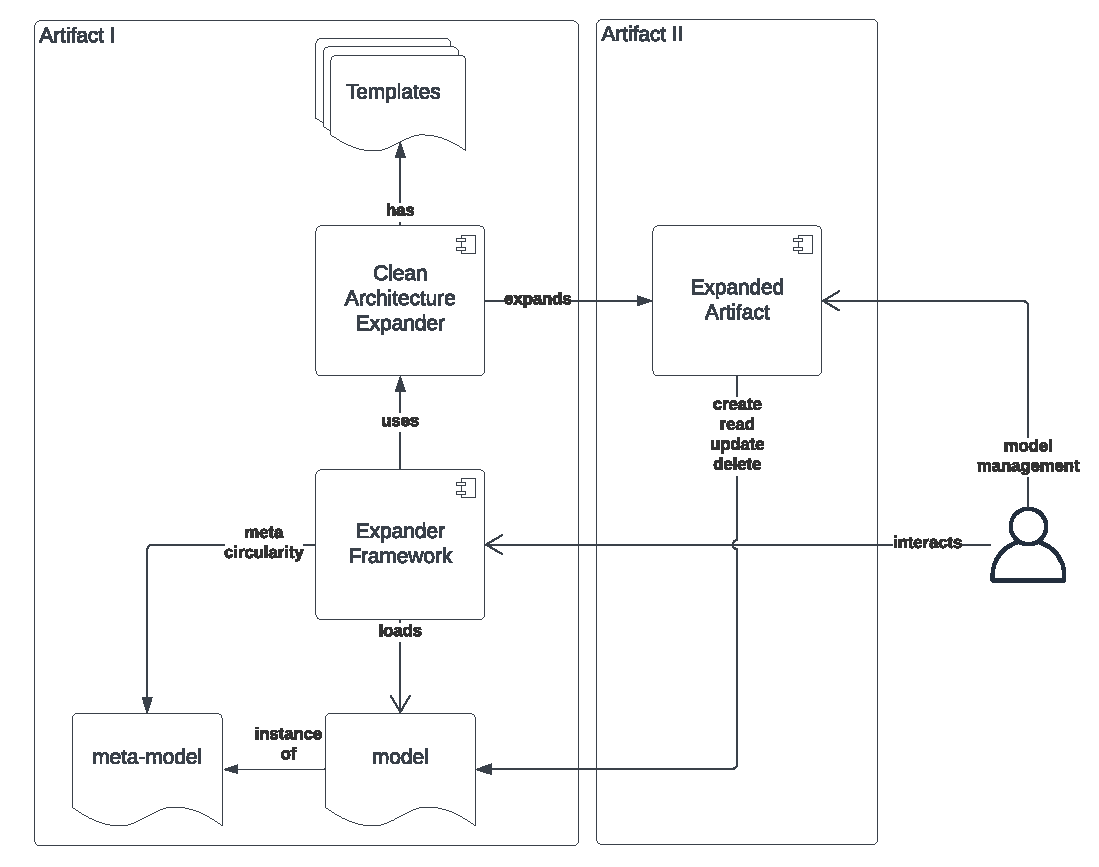
\includegraphics[width=0.8\textwidth]{figures/artifactOverview.pdf}
    \caption[Schematic overview of the Artifacts]{Schematic overview of the Artifacts}
    \label{fig_overview_design}
  \end{figure}

  As illustrated in Figure \ref{fig_overview_design}, the main task of the first artifact
  or \enquote*{expand} the second artifact. By entering the correct command, the Expander
  Framework loads the model being instantiated during the expansion process. Then, the
  required expanders are prepared based on information available through the model. In the
  case of this study, the Clean Architecture Expander. The Clean Architecture Expander
  consists of a set of tasks and templates. When the Expander Framework executes the Clean
  Architecture Expander, the model is instantiated into the generated artifact with the
  aid of the templates.

  The model is an instance of the meta-model. Consequently, the model can represent any
  application as long as the meta-model is respected. In the case of this study, the model
  represents the entities, attributes, relationships, and other characteristics of the
  meta-model.
  
  As a result, the second artifact (artifact II) allows a user to modify or maintain the
  model used by the Expander Framework by exposing a Restful interface. This method
  approaches the meta-circularity process, where an expansion process is used to
  update the meta-model. Although not fully compliant with the theory of \gls{ns}, the
  Expander Framework consists of the required tasks to update its own meta-model. This is
  illustrated in Figure \ref{fig_overview_design} by the \enquote*{updates} arrow.

\section{The Artifact name and use} \label{sec_artifact_name}

The name of the Expander Framework, Pantha Rhei, was inspired by the Greek philosopher
\emph{Heraclitus}, who famously stated that \enquote{life is flux}. The name reflects the
artifact's ability to cope with constant change in a stable and evolvable manner. The name
is also reflected in the use of the \enquote{flux} command in the \gls{cli}, which allows
users to interact with the application.

To install Pantha Rhei, interested readers can follow the instructions provided in the
appendix \fullref{koks_installation_2023}.





\chapter{The Entity Relationship Diagram of the Meta Mode} \label{appendix_metamodel_description}  

\section{The App entity}

The App entity represents the application and is regarded as the entry point for the
model. The App Entity and the subsequent entities contain all the information required to
perform the expandsion of a software system. 

\begin{table}[H]
    \small
    \begin{tabular}{ p{0.21\linewidth} p{0.21\linewidth} p{0.49\linewidth} }
        \hline
        \textbf{Name} & \textbf{DataType} & \textbf{Description} \\
        \hline
        Id & Guid & Unique identifier of the application \\
        Name & string & Name of the application \\
        FullName & string & Full name of the application \\
        Expanders & List of Expanders & The Expanders that will be used during the
        generation process. \\
        Entities & List of Entities & The Entities that are applicable for the Generated artifact. \\
        ConnectionStrings & List of ConnectionStrings & The ConnectionString to the
        database that is used by the Generator Artifact. \\
        \hline
    \end{tabular}
    \caption{The fields of the App entity}
    \label{table:app_entity}
\end{table}

\section{The Component entity}

The Component entity represents a software component that can be part of an application.
Based on this entity the Generator Artifact can make design time on where to place certain
elements  

\begin{table}[H]
\small
\begin{tabular}{ p{0.20\linewidth} p{0.20\linewidth} p{0.50\linewidth} }
\hline
\textbf{Name} & \textbf{DataType} & \textbf{Description} \\
\hline
Id & Guid & Unique identifier of the component \\
Name & string & Name of the component \\
Description & string & Description of the component \\
Packages & List of Package & The Packages that should be applied to the component. \\
Expander & Expander & Navigation property to the Expander entity. \\
\hline
\end{tabular}
\caption{The fields of the Component entity}
\label{table:component_entity}
\end{table}

\section{The ConnectionString entity}

The ConnectionString entity represents a ConnectionString used by an application to
connect to a database or other external system.

\begin{table}[H]
\small
\begin{tabular}{ p{0.20\linewidth} p{0.20\linewidth} p{0.50\linewidth} }
\hline
\textbf{Name} & \textbf{DataType} & \textbf{Description} \\
\hline
Id & Guid & Unique identifier of the ConnectionString \\
Name & string & Name of the ConnectionString \\
Definition & string & Definition of the ConnectionString \\
App & App & Navigation property to the App entity \\
\hline
\end{tabular}
\caption{The fields of the ConnectionString entity}
\label{table:connectionstring_entity}
\end{table}

\section{The Entity entity}

The Entity entity represents an entity in the application's data model. 

\begin{table}[H]
\small
\begin{tabular}{ p{0.20\linewidth} p{0.23\linewidth} p{0.47\linewidth} }
\hline
\textbf{Name} & \textbf{DataType} & \textbf{Description} \\
\hline
Id & Guid & Unique identifier of the entity \\
Name & string & Name of the entity \\
Callsite & string & The source code location where the entity is defined. In the case of a C\#
artifact, this is to determine the name of the namespace.\\
Type & string & Type of the entity \\
Modifier & string & Modifier of the entity (e.g. public, private) \\
Behavior & string & The behavior of the entity (e.g. abstract, virtual) \\
App & App & Navigation property to the App entity. \\
Fields & List of Fields & The Fields property represents a collection of the fields that
make up the entity. \\
ReferencedIn & List of Fields & Represents a navigation property to a Field that uses the
current entity as a return type. \\
Relations & List of Relationships & List of relationships involving this entity \\
IsForeignEntityOf & List of Relationships & List of relationships where this entity is the foreign entity \\
\hline
\end{tabular}
\caption{The fields of the Entity entity}
\label{table:entity_entity}
\end{table}

\section{The Expander entity}

The Expander entity represents an expander, which is responsible for generating code for
an application. The Generator Artifact attempts to execute all expanders that are related
to the selected App.

\begin{table}[H]
\small
\begin{tabular}{ p{0.20\linewidth} p{0.22\linewidth} p{0.48\linewidth} }
\hline
\textbf{Name} & \textbf{DataType} & \textbf{Description} \\
\hline
Id & Guid & Unique identifier of the expander \\
Name & string & Name of the expander \\
TemplateFolder & string & relative path to the templates that are used by the expander. \\
Order & int & The order in which the expander is executed \\
Apps & List of Apps & List of applications associated with the expander. \\
Components & List of Components & List of components associated with the expander \\
\hline
\end{tabular}
\caption{The fields of the Expander entity}
\label{table:expander_entity}
\end{table}

\section{The Field entity}

The Field entity represents a field or property of an entity in an application's data
model. Each field has a unique ID, name, and other properties such as its return type,
modifiers, and behavior. It can be associated with an entity and can have relationships
with other entities. The IsKey and IsIndex properties indicate whether the field is part
of the primary key or an index of the entity, respectively.

\begin{table}[H]
\small
\begin{tabular}{ p{0.23\linewidth} p{0.23\linewidth} p{0.45\linewidth} }
\hline
\textbf{Name} & \textbf{DataType} & \textbf{Description} \\
\hline
Id & Guid & Unique identifier of the field \\
Name & string & Name of the field \\
ReturnType & string & Return type of the field \\
IsCollection & bool & Whether the field is a collection or not \\
Modifier & string & Modifier of the field (e.g. public, private) \\
GetModifier & string & Modifier of the get accessor for the field \\
SetModifier & string & Modifier of the set accessor for the field \\
Behavior & string & The behavior of the field (e.g. abstract, virtual) \\
Order & int & The order of the field within its entity \\
Size & int? & The size of the field \\
Required & bool & Whether the field is required or not \\
Reference & Entity & The entity that this field refers to\\
Entity & Entity & A navigation property to the parent entity \\
IsKey & bool & Indicates whether the field is part of the primary key \\
IsIndex & bool & Indicates whether the field is part of an index \\
RelationshipKeys & List of Relationships & A List of entities that are defined as relations. \\
IsForeignEntityKeyOf & List of Relationships & List of relationships to the field that is the foreign key \\
\hline
\end{tabular}
\caption{The fields of the Field entity}
\label{table:field_entity}
\end{table}

\section{The Package entity}

The Package entity represents a software package that can be used by a component. This
could either be a Nuget package in the case of .NET projects, or for example npm packages
for web projects.

\begin{table}[H]
\small
\begin{tabular}{ p{0.20\linewidth} p{0.20\linewidth} p{0.50\linewidth} }
\hline
\textbf{Name} & \textbf{DataType} & \textbf{Description} \\
\hline
Id & Guid & Unique identifier of the package \\
Name & string & Name of the package \\
Version & string & Version of the package used \\
Component & Component & Component associated with the package \\
\hline
\end{tabular}
\caption{The fields of the Package entity}
\label{table:package_entity}
\end{table}

\section{The Relationship entity}

The Relationship entity represents a relationship between two entities in the App's data
model. The Relationship entity has proper cardinality support. Relationships are
bidirectional and can be navigated from either entity.

\begin{table}[H]
\small
\begin{tabular}{ p{0.24\linewidth} p{0.12\linewidth} p{0.55\linewidth} }
\hline
\textbf{Name} & \textbf{DataType} & \textbf{Description} \\
\hline
Id & Guid & Unique identifier of the relationship \\
Key & Field & The key field of the relationship \\
Entity & Entity & Navigation property to the parent Entity \\
Cardinality & string & The cardinality of the relationship \\
WithForeignEntityKey & Field & The foreign key field of the relationship, pointing to a
Field entity. \\
WithForeignEntity & Entity & The entity associated with the foreign key field \\
WithCardinality & string & The cardinality of the relationship with the foreign entity \\
Required & bool & indicates whether the relationship is required or not \\
\hline
\end{tabular}
\caption{The fields of the Relationship entity}
\label{table:relationship_entity}
\end{table}
\section{Plugin Architecture} \label{subsec_plugin_architecture}

The Expander Framework Artifact is responsible for loading and bootstrapping Expanders and
initiating the generation process. Expanders are dynamically loaded at runtime through a
dotnet capability called assembly binding, allowing the architecture illustrated in the
following image \parencite{koks_expanderpluginloaderinteractor_2023}.

\begin{figure}[H]
  \centering
  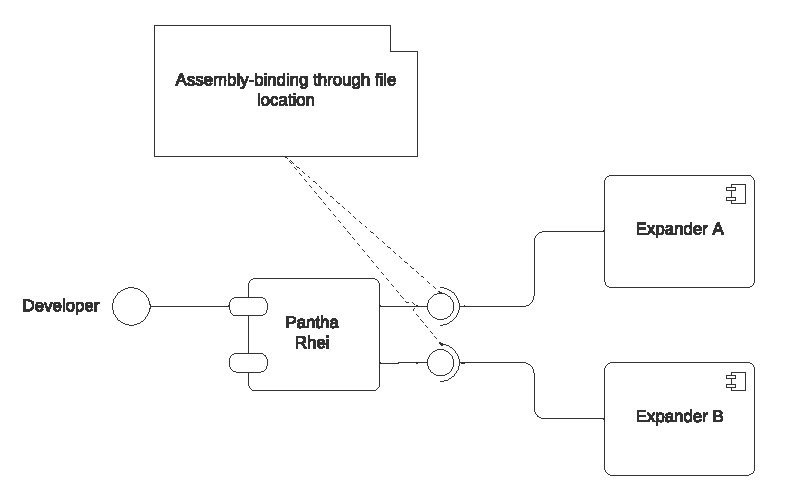
\includegraphics[width=0.5\textwidth]{figures/plugin_architecture.pdf}
  \caption[Plugin Archticture]{Expanders are considered plugins}
  \label{fi:plugin_architecture}
\end{figure}

This plugin design adheres to several principles of \gls{solid}. The \gls{srp} principle
is implemented by ensuring that an expander generates one and only one construct. The
\gls{ocp} principle is applied by allowing the creation of new expanders in addition to
the already existing ones. The \gls{lsp} principle is respected by enabling the addition
or replacement of expanders without modifying the internal workings of the Expander
Framework.

More details can be found in the Appendix \fullref{list_expanderpluginloaderinteractor}
\section{Expanders}

The Exander Framework allows for the miscellaneous execution of expanders of any type. The
Expander Framework is independent of any of the details of Expanders, fully adhering to
the principle of \gls{dip}. Conversely, an Expander is required to implement several
interfaces to ensure execution and dependency management are available during runtime. The
Expander Framework also consists of a set of default tasks, such as the execution of the
expansion tasks known as ExpanderHandlerInteractors
\citecode{koks_iexpanderhandlerinteractor_2023}, logging, bootstrapping dependencies, and
tasks to execute harvestings and injections. Except for the use of the
IExpanderInteractor, non of which are required.

Figure \ref{fig_expander_design} illustrates the dependencies between the domain layer of
the Expander Framework. The Clean Architecture Expander is considered an application layer
containing specific tasks bounded to a particular application or process. In this case,
the Expansion process.

\begin{figure}[H]
    \centering
    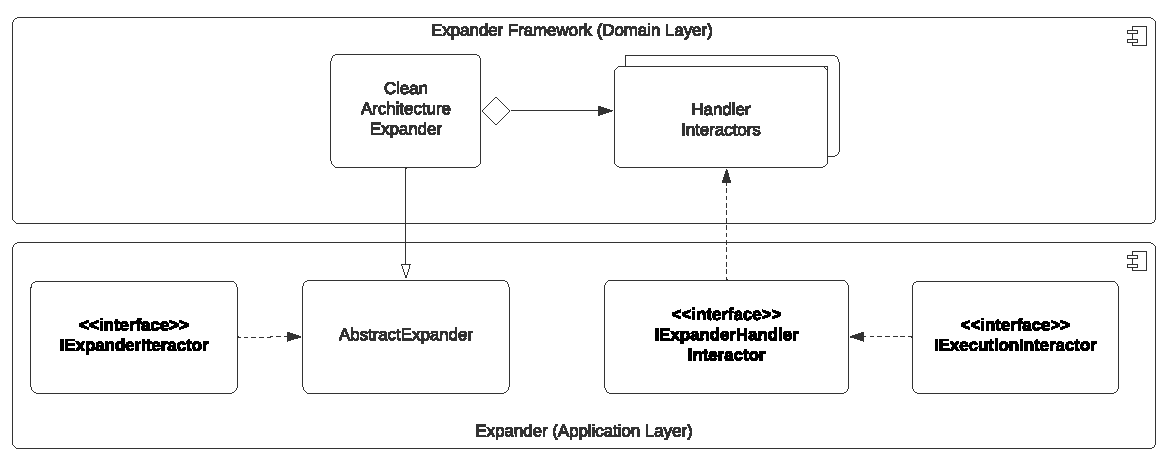
\includegraphics[width=1\textwidth]{figures/expander.pdf}
    \caption[The design of an Expander]{The design of an Expander}
    \label{fig_expander_design}
  \end{figure}
\section{The IExecutionInteractor command} \label{subsec_IExecutionInteractorObject}

An exciting implementation that facilitates a high degree of cohesion while maintaining
low coupling is the utilization of the \code{koks_iexecutioninteractor_2023} interface
\parencite{koks_iexecutioninteractor_2023}. This interface allows for the execution of
various derived types responsible for specific tasks, such as executing Handlers,
Harvesters, and Rejuvenators \parencites{koks_expandentitieshandlerinteractor_2023,
koks_regionharvesterinteractor_2023, koks_regionrejuvenatorinteractor_2023}. The
implementation promotes decoupling by adhering to both \gls{ocp} and \gls{lsp}.

\begin{figure}[H]
    \centering
    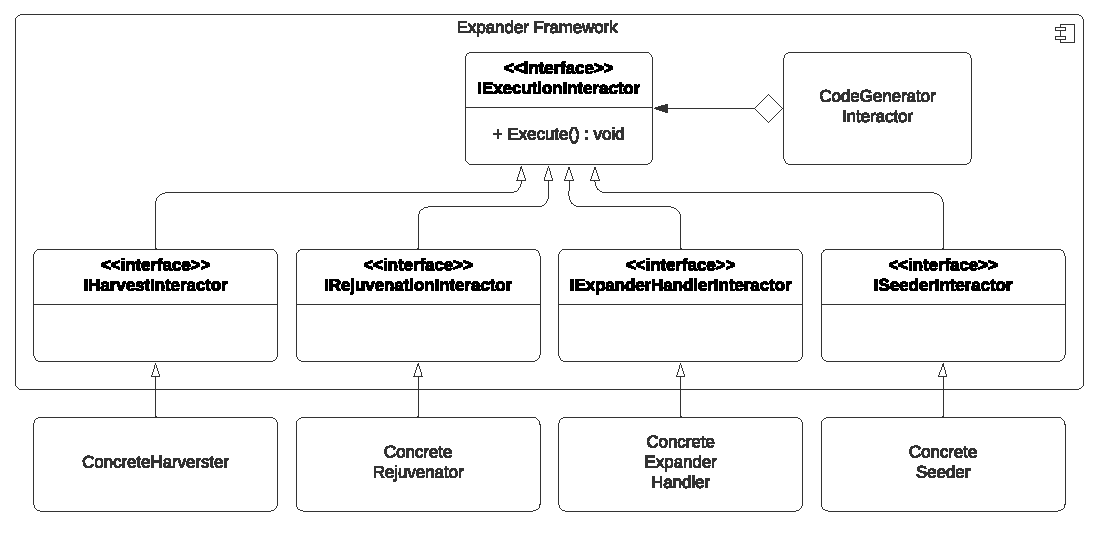
\includegraphics[width=1\textwidth]{figures/command_pattern.pdf}
    \caption[Low coupling with \code{koks_iexecutioninteractor_2023}]{Low coupling with \code{koks_iexecutioninteractor_2023}}
    \label{fig_iexecutioninteractor}
  \end{figure}


Figure \ref{fig_iexecutioninteractor} illustrates that the required interfaces are placed
in the Domain Layer of the Expander Framework. In contrast, the concrete classes also can
be implemented as part of the internal scope of the Clean Architecture Expander
\parencite{koks_migrationharvesterinteractor_2023}. Code listing
\fullref{list_expandentitieshandlerinteractor} illustrates an implementation example of
this interface. Finally, the code listing \fullref{list_CodeGeneratorInteractor}
illustrates the aggregation of the execution, which allows for a graceful cohesion of the
execution Tasks \parencite{koks_codegeneratorinteractor_2023}.

\section{Dependency management}

\begin{enumerate}
    \color{red}
    \item TODO: DESCRIBE DI and use of service locator pattern.
\end{enumerate}
\chapter{Evaluation results} \label{chap_evaluation}

\section{Converging principles} \label{sec:converging_principles}

In order to address \nameref{rq3} outlined in Chapter \ref{sec:research_questions}, a
comprehensive analysis of the existing literature on the \gls{solid} principles and
\gls{ns} theorems have been conducted. Furthermore, the development of the artifact has
provided valuable insights into this subject matter.

In the following sections, a systematic cross-referencing approach has been applied to
assess the level of convergence between each of the \gls{solid} principles of \gls{ca}
and the \gls{ns} theorems. Along with a brief explanation, the level of convergence is
denoted as follows:

\begin{table}[H]
    \begin{tabular}{ l l p{0.57\linewidth}} Fully converges & \converges & This indicates
        a high degree of alignment between the respective \gls{solid} principle and
        \gls{ns} theorem. The application of either principle or theorem results in a
        similar impact on the software design. \\
        Supports convergence & \supports & In this case, the \gls{solid} principle
        assists in implementing the \gls{ns} theorem through specific design choices.
        However, it is essential to note that applying the principle does
        not inherently ensure adherence to the corresponding theorem. \\
        No convergence & \diverges & This denotation signifies a lack of alignment between
        the \gls{solid} principle and the corresponding theorem. \\
    \end{tabular}
\end{table}

\subsection{The convergence of the Single Responsibility Principle}

\begin{table}[H]
    \begin{tabular}{ l | c | p{0.78\linewidth}}
        \toprule
        \gls{soc} & \converges & \gls{srp} and \gls{soc} share a common objective:
        facilitating evolvable software systems through the promotion of modularity, low
        coupling, and high cohesion. While there may be some differences in granularity
        when applying both principles according to the original definition of SOC, the
        more stringent definition of Separation of Concerns, offered by the \gls{ns}
        Theorems \ref{subsubsec:soc} minimizes these differences. As a result, the two
        principles can be regarded as practically interchangeable. In conclusion, SRP and
        SOC exhibit full convergence, as they both emphasize encapsulating
        'responsibilities' or 'concerns' within modular components of a software system.
        \\
        \midrule
        \gls{dvt} & \supports & While not immediately obvious, \gls{srp} offers supports
        for the \gls{dvt} theorem. While \gls{srp} emphasizes limiting the responsibility of
        each module, it does not explicitly require handling changes in data structures.
        However, following gls{srp} can still indirectly contribute to achieving \gls{dvt}
        by promoting the Law of Demeter
        \footnote{\url{https://en.wikipedia.org/wiki/Law_of_Demeter}}, which encourages
        modules to interact with each other only through well-defined interfaces. This
        approach can minimize the impact of data structure changes, although it does not
        guarantee full convergence with \gls{dvt}. \\
        \midrule
        \gls{avt} & \supports & Although not that apparent, \gls{srp} supports the \gls{dvt}
        theorem. While \gls{srp} emphasizes limiting the responsibility of each module, it
        does not explicitly require handling changes in data structures. However, following
        gls{srp} can still indirectly contribute to achieving \gls{dvt} by promoting the Law
        of Demeter \footnote{\url{https://en.wikipedia.org/wiki/Law_of_Demeter}}, which
        encourages modules to interact with each other only through well-defined interfaces.
        This approach can minimize the impact of data structure changes, although it does not
        guarantee full convergence with \gls{dvt}. \\
        \midrule
        \gls{sos} & \diverges & The convergence between \gls{srp} and the \gls{sos} theorem is
        not as direct as with other theorems. \gls{srp} focuses on assigning a single
        responsibility to each module but does not explicitly address state management.
        Nevertheless, by following \gls{srp}, developers can create modules that manage their
        state, which indirectly contributes to \gls{sos}. \\
        \bottomrule
    \end{tabular}
    \caption{Convergence \gls{srp} with \gls{ns}}
    \label{tab:convergence_srp}
\end{table}

\subsection{The convergence of the Open/Closed Principle}

\begin{table}[H]
    \begin{tabular}{ l | c | p{0.78\linewidth}}
        \toprule
        \gls{soc} & \converges & The \gls{ocp} converges with the \gls{soc} theorem.
        \gls{ocp} states that software implementations should be open for extension but
        closed for modification. When applying \gls{ocp} correctly, modifications are
        separated from the original implementations. For example by creating a new
        implementation of an interface or a base class. Conversely, adhering to \gls{soc}
        does not guarantee the fulfillment of \gls{ocp}, as \gls{soc} focuses on
        modularization and encapsulation, rather than the extensibility of modules. \\
        \midrule
        \gls{dvt} & \supports & The \gls{ocp} supports the \gls{dvt} theorem. While
        \gls{dvt} aims to handle changes in data structures without impacting the system,
        \gls{ocp} focuses on the extensibility of software entities. \gls{ocp} does not
        explicitly address data versioning, and thus does not guarantee full convergence
        with \gls{dvt}. However, by designing modules that follow \gls{ocp}, developers
        can create components that are more adaptable to changes in data structures. \\
        \midrule
        \gls{avt} & \converges & The \gls{ocp} converges with the \gls{avt} theorem. Both
        principles emphasize the importance of allowing changes or extensions to actions
        or operations without modifying existing implementations. By adhering to
        \gls{ocp}, developers can create modules that can be extended to accommodate new
        actions or changes in existing ones, effectively achieving \gls{avt}. \\
        \midrule
        \gls{sos} & \diverges & The \gls{ocp} has an indirect relationship with the
        Separation of States (SoSt) theorem. but not on a level where we can speak of
        convergence. \gls{sos} emphasizes isolating different states within a system.
        Adhering to \gls{ocp} alone does not guarantee full separation of states. \\
        \bottomrule
    \end{tabular}
    \caption{Convergence \gls{ocp} with \gls{ns}}
    \label{tab:convergence_ocp}
\end{table}
\subsection{The convergence of the Liskov Substitution Principle}

\begin{table}[H]
    \begin{tabular}{ l | c | p{0.78\linewidth}}
        \toprule
        Theo & Conv & Desc \\
        \midrule
        \gls{soc} & \converges & Adhering to \gls{lsp} in the software design leads to a more
        modular design and separation of certain concerns. Therefore we state that \gls{lsp}
        converges with \gls{soc}. \gls{lsp} states that objects of a derived class should be
        able to replace objects of the base class without affecting the correctness of the
        program. This can only be achieved by a strict separation of concerns in combination
        with Action version Transparent implementations of the signature.
        \\
        \midrule
        \gls{dvt} & \converges & \gls{lsp} has a (limited) support for the \gls{dvt} theorem.
        While \gls{lsp} focuses on the substitutability of objects in class hierarchies,
        \gls{dvt} aims to handle changes in data structures without impacting the system. By
        following \gls{lsp}, developers can ensure that derived classes can be substituted for
        their base classes, which may help reduce the impact of data structure changes on the
        system. However, \gls{lsp} does not explicitly address data versioning and thus does
        not guarantee full convergence with \gls{dvt}. 
        \\
        \midrule
        \gls{avt} & \converges & The \gls{lsp} supports the \gls{avt} theorem. Both principles
        emphasize the importance of allowing the extensibility of the system, without
        negatively impacting the desired requirements. By adhering to \gls{lsp}, developers
        can create class hierarchies that can be easily extended to accommodate new actions or
        changes in existing ones, which may contribute to achieving \gls{avt}. However,
        adhering to \gls{lsp} alone may not guarantee full convergence with \gls{avt}. 
        \\
        \midrule
        \gls{sos} & \converges & By designing class hierarchies according to \gls{lsp},
        developers can create components that are less prone to side effects caused by shared
        states. However, the alignment between \gls{lsp} and \gls{sos} is very weak, and
        adhering to \gls{lsp} alone may not guarantee full separation of states. 
        \\
        \bottomrule
    \end{tabular}
    \caption{Convergence \gls{lsp} with \gls{ns}}
    \label{tab:convergence_lsp}
\end{table}
\subsection{The convergence of the Interface Segregation Principle}

\begin{table}[H]
    \begin{tabular}{ l | c | p{0.78\linewidth}}
        \toprule
        \gls{soc} & \converges & The \gls{isp} converges with the \gls{soc} theorem, as
        both principles emphasize the importance of modularity and the separation of
        concerns. \gls{isp} states that clients should not be forced to depend on
        implementation they do not use, promoting the creation of smaller, focused
        interfaces. By adhering to \gls{soc} and designing target interfaces, inherently
        support \gls{soc}, leading to more evolvable software systems. \\
        \midrule
        \gls{dvt} & \supports & The \gls{isp} has an indirect relationship with the
        \gls{dvt} theorem. When adhering to the \gls{isp}, a developer can create a
        specific interface supporting a specific version of data entities. Although this
        approach can help minimize the impact of data structure changes on the system, it
        does not guarantee full \gls{dvt} information system. \\
        \midrule
        \gls{avt} & \supports & The \gls{isp} supports the \gls{avt} theorem. Both
        principles emphasize the importance of separating actions within a system.
        \gls{isp} promotes the creation of interfaces for each (version of an) action,
        which aligns with the core concept of \gls{avt}. This alignment allows for a more
        manageable system, where changes in one action do not lead to ripple effects
        throughout the entire system. Although the adherence to \gls{isp} does not
        guarantee full compliance with the \gls{avt} \\
        \midrule
        \gls{sos} & \diverges &  There is no alignment between \gls{isp} and \gls{sos}.
        Mostly because \gls{isp} focuses on the separation of interfaces and abstract
        classes, while \gls{sos} emphasizes isolating different states within a system.
        This is an implementation concern. By no means the application of \gls{isp} could
        lead to a separation of state. \\
        \bottomrule
    \end{tabular}
    \caption{Convergence \gls{isp} with \gls{ns}}
    \label{tab:convergence_isp}
\end{table}
\subsection{The convergence of the Interface Segregation Principle}

\begin{table}[H]
    \begin{tabular}{ l | c | p{0.78\linewidth}}
        \toprule
        \gls{soc} & \converges & This principle converges with the \gls{soc} theorem.
        \gls{dip} states that high-level modules should not depend on low-level modules.
        When unavoidable, high-level modules should depend on abstractions of low-level
        modules and abstractions should not depend on details. By adhering to \gls{dip}
        correctly, developers can create modular and decoupled software systems, which
        aligns to break down a system into evolvable components. This convergence enables
        developers to create maintainable, scalable, and adaptable software systems that
        effectively manage complexity. Dependency Injection is a valuable (but not the
        only or mandatory) aspect of \gls{dip}. We have observed that the claim that the
        technique of Dependency Injection solves coupling between classes in an
        application is dangerous and in some cases wrong
        \parencite[215]{mannaert_normalized_2016}. Nevertheless, this technique, when
        applied correctly (see ref{subsubsec:dip}), the artifact have pointed out that it
        has been a great asset in creating evolvable software, especially in the aspect of
        \gls{soc}.\\
        \midrule
        \gls{dvt} & \supports &  Adhering to the \gls{dip} can indirectly support the
        \gls{dvt} theorem. By adhering to the \gls{dip}, developers can promote
        implementations that encourage modules to interact with each other only through
        well-defined interfaces or abstractions. This approach can help minimize the
        impact of data structure changes on the system but does not guarantee full
        compliance with \gls{dvt}. \\
        \midrule
        \gls{avt} & \supports & The \gls{dip} can support the \gls{avt} theorem. Both
        principles emphasize the importance of isolating actions or operations within a
        system. By adhering to \gls{dip}, developers can create modular components that
        interact through abstractions, which may contribute to achieving AvT. However, the
        alignment between \gls{dip} and \gls{avt} less strong than with \gls{soc}, and
        adhering to \gls{dip} alone will not guarantee a system that entirely complies to
        \gls{avt}. \\ 
        \midrule
        \gls{sos} & \diverges & There is a very weak alignment between \gls{dip} and
        \gls{sos}. Although Developers can create components that are less prone to side
        effects caused by a shared state, this can hardly be contributed to the \gls{dip}.
        Therefore it is stated that there is no convergence between the two principles.\\
        \bottomrule
    \end{tabular}
    \caption{Convergence \gls{dip} with \gls{ns}}
    \label{tab:convergence_dip}
\end{table}
\section{Conclusion}

\begin{table}[!ht]
    \centering
    \begin{tabular}{lcccc}
    \toprule
     & SoC & DVT & AVT & SoS \\
    \midrule
    SRP & \converges & \supports & \supports & \diverges \\
    OCP & \converges & \supports & \converges & \diverges \\
    LSP & \converges & \diverges & \supports & \diverges \\
    ISP & \converges & \supports & \supports & \diverges \\
    DIP & \converges & \supports & \supports & \diverges \\
    \bottomrule
    \end{tabular}
    \caption{Convergence between SOLID principles and Normalized Systems theorems (abbreviated)}
    \label{tab:convergence_abbreviated}
    \end{table}


\chapter{Discussion} \label{discussion}
\chapter{Conclusions and discussion} \label{chap_conclusions}

This thesis embodies a multidimensional exploration of the convergence of \gls{ca} with
\gls{ns}. We have drawn upon the author's firsthand experience designing software
architectures using rigorous theoretical research. Additionally we created practical and
working software artifacts. The primary objective was to study the convergence between
\gls{ca} and \gls{ns} by analyzing their principles and design elements through theory
and practice. This chapter will summarize the findings into a research conclusion.

\section{Conclusion}

A noteworthy distinction between \gls{ns} and \gls{ca} lies in their foundational roots.
\gls{ns} is a product of computer science research built upon formal theories and
principles derived from rigorous scientific investigation. Although, throughout this
thesis, \gls{ns} is referred to as a development approach, it is actually a part of
Computer Science.

Stability and evolvability are concepts not directly referenced in the literature on
\gls{ca}, but this design approach aligns with the goal of
\textcite[31]{mannaert_normalized_2016}. As depicted in Table
\ref{tab_convergence_principles_summarized}, the attentive reader surely observes the
shared emphasis on modularity and the separation of concerns, as all SOLID principles have
a strong convergence with \gls{soc}. Both approaches attempt to achieve low coupling and
high cohesion. In addition, \gls{ca} adds the dimensions of dependency management as
useful measures to improve maintainability and manage dependencies in a modular
architecture.

The Transparency of Data versions appears to be underrepresented in the SOLID principles
of \gls{ca}. \gls{dvt} is primarily supported by the \gls{srp} of \gls{ca}, as evidenced
by the presence of ViewModels, RequestModels, ResponseModels, and Entities in the
artifact. It is worth noting that this separation of concerns on an ontological level is an
integral part of the design elements of \gls{ca}. While \gls{ca} does address \gls{dvt}
through the \gls{srp}, a more comprehensive representation of the underlying idea of
\gls{dvt} within the principles of \gls{ca} will likely improve the convergence of
\gls{ca} with \gls{ns}, potentially improving the stability and evolvability of software
Systems based on \gls{ca}.

As described in section \ref{combinatorics}, the underrepresentation of \gls{dvt} has
led to significant combinatorial effects in some parts of the artifacts. These
combinatorial effects are also be attributed to the author's inexperience in creating
systems that enable code generation through expansion while maintaining stability on
templates and craftings. When Data Version Transparency was better represented in the
principles of \gls{ca}, the severity of the combinatorial effects would have most likely
been less.

As indicated in Table \ref{tab_convergence_elements_summarized}, \gls{ca} lacks a strong
foundation for receiving external triggers in its design philosophy. This is partially
represented by the Controller element. However, this element tends to be used for
web-enabled environments like websites and Restful APIs. This may result in a less
comprehensive approach to receiving external triggers across various technologies or
systems.

The most notable difference between \gls{ca} and \gls{ns} is their approach to handling
state. \gls{ca} does not explicitly address state management in its principles or design
elements. At the same time, \gls{ns} provides the principle of Separation of State,
ensuring that state changes within a software system are stable and evolvable. This
principle can be crucial in developing scalable and high-performance systems, as it
isolates state changes from the rest of the system, reducing the impact of state-related
dependencies and side effects. 

The findings can only lead to the conclusion that the convergence between \gls{ca} and
\gls{ns} is incomplete because \gls{ca} needs specific state management principles. As a
result, \gls{ca} cannot fully ensure stable and evolvable software artifacts as defined by
\gls{ns}.



\section{Discussion}

In this research, the convergence between \gls{ca} and \gls{ns} has been thoroughly
investigated. While it has been demonstrated that the convergence between these two
approaches is incomplete, combining both methodologies is highly beneficial for both
\gls{ns} as for \gls{ca} for various reasons. The primary advantage of this convergence
lies in the complementary nature of \gls{ca} with \gls{ns}, where each approach provides
strengths that can be leveraged to address a strong architectural design. 

Clean Architecture offers a well-defined, practical, and modular structure for software
development. Its principles, such as SOLID, guide developers in creating maintainable,
testable, and scalable systems. This architectural design approach is highly suitable for
various applications and can be easily integrated with the theoretical foundations
provided by \gls{ns}. 

Conversely, the NS approach offers a more comprehensive theoretical understanding of
achieving stable and evolvable systems. Furthermore, the popularity and widespread
adoption of Clean Architecture in the software development community can benefit
Normalized Systems. As more developers already adopting \acrlong{ca} become more familiar
with \acrlong{ns} and recognize its value to software design. Combining both approaches
will likely lead to increased adoption of \acrlong{ns}.
\section{Limitations}

In this research, the artifacts created to demonstrate the convergence between \gls{ca}
and \gls{ns} have shown promising results. However, it is essential to recognize these
artifacts' limitations, particularly in implementing \gls{ns} principles such as the
Separation of State Principle and the Trigger Element. These limitations must be
acknowledged to guide future work and refinement of the combined architectural design
approaches.

One of the primary limitations of the artifacts lies in their incomplete representation of
the Separation of State principle. This principle is crucial in \gls{ns} to ensure proper
handling of state changes while achieving stability and evolvability. While the artifacts
incorporate some aspects of state management, they fall short of fully implementing the
Separation of State principle as \gls{ns} prescribes. 

The other limitation of the artifacts is their lack of a comprehensive Trigger Element, an
essential element of \gls{ns}. The Trigger Element manages external triggers while
ensuring that software remains stable and evolvable. In the artifacts, incorporating the
Trigger Element is limited, primarily relying on the Controller element from \gls{ca}.
While this approach may be sufficient for web-enabled environments such as websites and
RESTful APIs, it may not be adequate for a broader range of requirements.
\section{Reflections} \label{chap_reflection}

This section will dive into my enriching experiences and invaluable learnings acquired
while working on this research and thesis and is inspired by one of the master classes
about the \gls{ee} discipline. \gls{ee} encourages using grounded methodologies and
theories, like Five Way Framework, to comprehend the inner workings of an enterprise
\parencite[262]{dietz_enterprise_2020}. I will apply the so-called Five Way Framework to
reflect on this research. By incorporating the Five Way Framework into the section, I
aspire to coherently showcase my learnings and reflections, shedding light on my thought
processes, strategies, modeling techniques, working methodologies, and support mechanisms.

\begin{figure}[H]
    \centering
    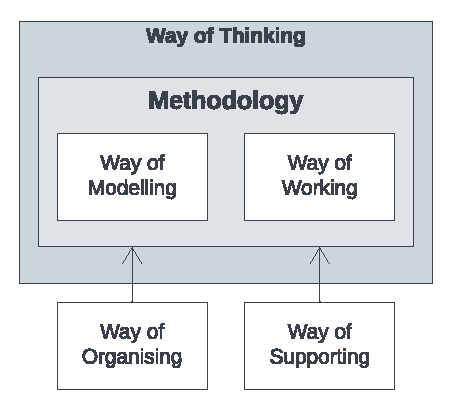
\includegraphics[width=0.5\textwidth]{figures/5ways.pdf}
    \caption[The Five Way Framework]{The Five Way Framework, inspired by \textcite{dietz_enterprise_2020}}
    \label{fig_5ways}
\end{figure}

\subsection{Way of Thinking}

Early in my career, I became obsessed with Software Quality and Maintainability. The
\gls{ns} theory shifted the obsession toward Stability and Evolvability. Gaining a
thorough understanding of the essential principles of this theory has boosted my
confidence in making informed decisions regarding all aspects of architecture, not just
limited to software.

As a Domain Architect, my job involved creating software products using the \gls{mdd}
paradigm. Initially, I was skeptical about this approach based on my early experiences.
The theory of \gls{ns} taught me to understand better the reasoning and characteristics of
code generation, on which I then realized that my skepticism was more about the process
caused as an effect on the implementation of the \gls{mdd}. The knowledge of \gls{ns}
helped me gain a clearer vision and helped me push the roadmap on the \gls{mdd} framework
in the right direction.

\subsection{Way of Modeling}

To explain the implementation concepts of the artifact, I looked into various modeling
languages. Archimate was the first option I considered. However, during one of the \gls{ee}
masterclasses, I learned the hard way that Archimate is not always the best choice for
communicating your models to a broad audience. I thought about using basic "boxes and
arrows" but decided to use the UML2 standard because it is a formal modeling language.

\subsection{Way of Working}

I very much enjoyed designing and creating the C\# artifacts. In hindsight, I enjoyed it
so much that I put in way too much effort than was needed. I was very curious about the
aspects of code generation, the effect of code generation on stable and evolvable
artifacts, and meta-circularity characteristics. I am confident I could have arrived at
the same conclusions presented in this thesis using a manually built Restful C\# artifact.
However, the insights I gained on the subjects of code expansion are of invaluable value
to me. Therefore, I am very pleased and satisfied that I took the effort to build the Code
Expander as a primary artifact. 

The \gls{ns} theorems are formulated very clearly and abstractly, making them also
applicable outside the software engineering field. During the masterclasses, we learned
about the application of \gls{ns} in the domains of Firewalls, Document management
systems, and Evolvable Business Processes. I also experienced benefits in structuring and
maintaining my Thesis document using \gls{vscode} and Latex by applying the principle of
\gls{soc} in managing the various chapters and sections. 

\subsection{Way of Organizing}

I should have been able to finish sooner. I was one of the first with a research topic and
started working on my artifact in the first month when starting this journey. The artifact
was as good as ready before the summer holidays of the first year. Unfortunately, I
postponed writing the thesis until a later moment. I want to think that next time I will
start sooner, but knowing myself, I need some pressure to perform the less fun tasks, like
writing this thesis.

The review process seemed difficult and sometimes even problematic for a couple of
reasons. Next time I will ensure having the proper tools and agree on procedures to
improve reviews from multiple proofreaders. Secondly, I noticed that having multiple
proofreaders sometimes steers in opposite directions. This sometimes affected my ability
to make decisions and negatively affected my confidence. Having a joined review document,
where all proofreaders can leave comments, will significantly improve this experience for
me and my proofreaders. Then there is the personal aspect of sometimes taking things too
personally, grounded in a lack of self-confidence. However, this experience improved my
self-confidence. 

\subsection{Way of Supporting}

At the beginning of my research, I received a thorough introduction to the \gls{ns}
Theories and the Prime Radiant tooling from an employer at NSX. This introduction was
extremely helpful in gaining a better understanding of the fundamentals of \gls{ns}. It
also inspired me to consider the Code Expansion as a primary artifact. 

For the writing of the Thesis, I decided to use Latex. I quickly discovered that Overleaf
was one of the most popular editors. Nevertheless, I continued my search since I rejected
the idea of relying on online tooling for writing my Thesis. At some point, I decided to
experiment with my favorite code editor \gls{vscode}, and with the help of a latex package
manager and some \gls{vscode} plugins, I was able to create a fully-fledged Latex Editor
in \gls{vscode}, being able to use all the other benefits that come with \gls{vscode}. In
my next project, I will likely use the \gls{vscode} Latex editor again.



%----------------------------------------------------------------------------------------
%	THESIS CONTENT - APPENDICES
%----------------------------------------------------------------------------------------

\appendix % Cue to tell LaTeX that the following "chapters" are Appendices

% Include the appendices of the thesis as separate files from the Appendices folder
% Uncomment the lines as you write the Appendices

%\include{Appendices/Erd.tex}
\chapter{The Entity Relationship Diagram of the Meta Mode} \label{appendix_erd}  
\begin{figure}[H]
    \centering
    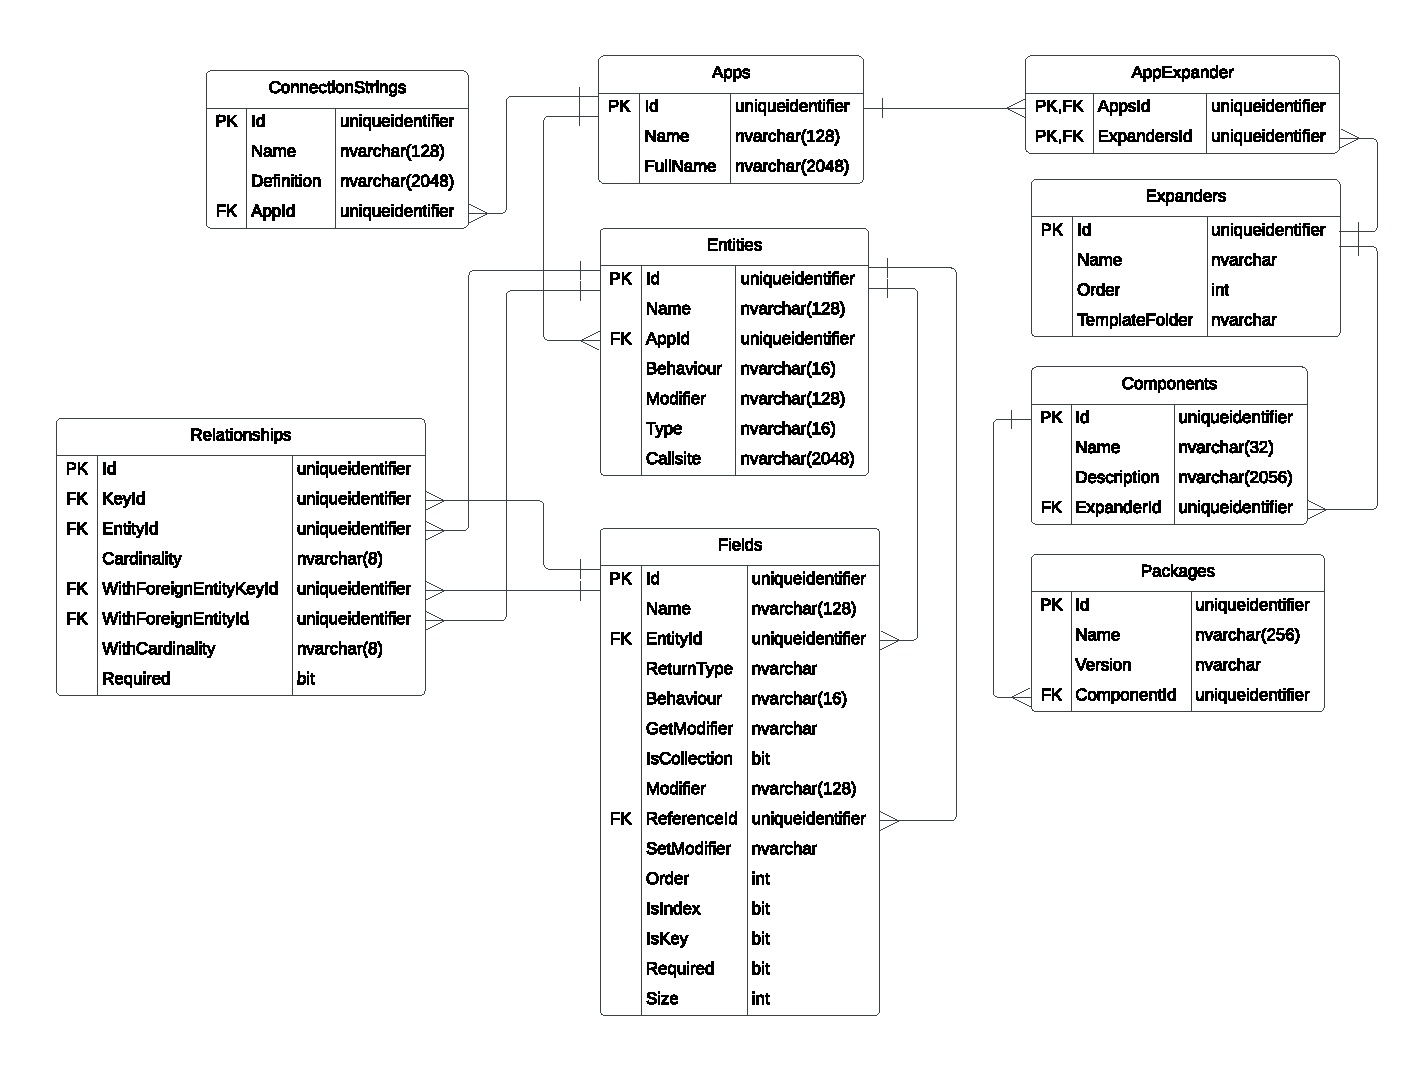
\includegraphics[width=1\textwidth]{Figures/erd.pdf}
    \caption[ERD]{Entity Relationship Diagram of the MetaModel}
    \label{fig_erd}
\end{figure}

\chapter{Installing \& using Pantha Rhei} \label{appendix_installation_instructions} 

\section{Installation instructions} \label{appendix_installation_prerequisits}
\subsection*{Step 1: Create output folder}
Create an output folder so that the applications...
\begin{itemize}
    \item ...has a location where to find the required expanders.
    \item ...has a location where the log files are stored.
    \item ...has a location where the result of the generation processes can be stored.
\end{itemize}

The location of the output folder is irrelevant.

\subsection*{Step 2: Create the Nuget configuration file}
Add a configuration file named \emph{nuget.config} file to the output folder with the
the following content: 

\lstinputlisting[ caption={The content of the Nuget configuration file},
label={list_nugetconfig}] {Snippets/nuget.config}

This config file is needed for the following step where the Pantha Rhei application is
installed. The file contains the information to the private feed where the Pantha Rhei
application can be downloaded and installed.

\subsection{Step 3: Installing Pantha Rhei} \label{appendix_installing_pantha_rhei} 
Open a console in on the location where the Nuget configuration file is stored. The
following command will download the package, and start the installation process which is
executed in the background. 

\lstinputlisting[
    caption={The install command},
    label={list_install-command}]
    {Snippets/dotnet-install-command.txt}

\subsection*{Step 4: Download \& Install the Expanders}
By clicking on the following link, an archived folder will be presented as a download by
your browser. Download the archived folder and extract it on completion. Store the
extracted folder, in a subfolder called \emph{Expanders} in the root of the output
folder. By doing so, the following folder structure should be available:

\begin{forest}
    for tree={
      font=\ttfamily,
      grow'=0,
      child anchor=west,
      parent anchor=south,
      anchor=west,
      calign=first,
      inner xsep=7pt,
      edge path={
        \noexpand\path [draw, \forestoption{edge}]
        (!u.south west) +(7.5pt,0) |- (.child anchor) pic {folder} \forestoption{edge label};
      },
      % style for your file node 
      file/.style={edge path={\noexpand\path [draw, \forestoption{edge}]
        (!u.south west) +(7.5pt,0) |- (.child anchor) \forestoption{edge label};},
        inner xsep=2pt,font=\small\ttfamily
                   },
      before typesetting nodes={
        if n=1
          {insert before={[,phantom]}}
          {}
      },
      fit=band,
      before computing xy={l=15pt},
    }  
    [PanthaRhei.Output
    [Expanders
        [.Templates]
    ]
    [nuget.config, file]
  ]
\end{forest}

The Pantha Rhei application is now ready for use.

\subsection*{Setup a SQL database}
Currently, Pantha Rhei is working with an MS SQL database for storing the model of the
applications. Set up a SQL Database. This can either be a licensed version of SQL Server,
the free-to-use SQL Express or an Azure SQL instance. See
\url{https://www.microsoft.com/en/sql-server/sql-server-downloads} for more information.
Make sure to have a valid connection string to the SQL server instance that is needed in
step \fullref{appendix_run_flux}.

\section{Commandline manual} \label{appendix_run_flux}

Pantha Rhei is used by executing the \emph{flux} command with the following parameters

\begin{table}[H]
    \begin{tabular}{ l | p{0.78\linewidth}}
        \toprule
        --root & A mandatory parameter that should contain the full path to the output
        directory \fullref{appendix_installation_instructions}. \\
        --db & A mandatory parameter that contains the connectionstring to the database. \\
        --app & A mandatory parameter indicating the unique identifier of the application that should be generated. \\
        --mode & An optional parameter that determines if a handler should be executed.
        \emph{Default} is the default fallback mode (see \ref{tab:generation_modes}). \\
        --reseed & An optional parameter that bypasses the expanding process. The model will
        be thoroughly cleaned, and reseeded based on the entities of the expander
        artifact. This enables to a certain extent the meta-circularity and enables the
        expander artifact to generate itself. \\
        \bottomrule
    \end{tabular}
    \caption{The \emph{flux} command line parameters}
    \label{tab:commandline_parameters}
\end{table}

\lstinputlisting[
    caption={Example command executing Pantha Rhei},
    label={list_flux}]
    {Snippets/flux.txt}

RunModes are available to isolate the execution of the ExpanderHandler. It
requires a current implementation shown in listing \ref{list_runmode_example}. The
following RunModes are available.

\begin{table}[H]
    \begin{tabular}{ l | p{0.78\linewidth}}
        \toprule
        Default & This is the default generation mode that executes all configured
        handlers of the CleanArchitectureExpander. This will also install the required
        Visual Studio templates which are needed for scaffolding the Solution and C\#
        Project files. Furthermore, it also executes the Harvest and Rejuvenation
        handlers. This mode will clean up the entire output folder prior after the
        Harvesting process is finished prior to the execution of the handlers. \\
        
        Extend & This mode will skip the installation of the Visual Studio templates and
        the project scaffolding. It will not clean up the output folder but will
        overwrite any files handled. This mode is often less time-consuming and can be
        used in scenarios to quickly check the result of a part of the generation process. \\

       Deploy & An optional mode that allows for expander handlers to run deployments in
       isolation. For example, when a developer wants to deploy the output to an Azure App
       Service. \\
       
       Migrate & An optional mode that allows for expander handlers to run migrations in
       isolation. For example, this  currently updates the database schema by running the
       Entity Framework Commandline Interface (see \url{https://learn.microsoft.com/en-us/ef/core/cli/dotnet}).\\
        \bottomrule
    \end{tabular}
    \caption{The available \emph{Generation modes}}
    \label{tab:generation_modes}
\end{table}

\lstinputlisting[
    caption={Example on how an expander handler can adhere to the RunMode parameters},
    label={list_runmode_example}]
    {Snippets/RunModeExample.cs}



\chapter{Designs \& architecture} \label{appendix_designs} 

\section{Component layer naming conventions} \label{appendix_component_naming_convention}

\textbf{[PROD]} is defined as \textit{The name of the product of the software.} \newline 
\textbf{[COMP]} is defined as \textit{The name of the Company that is considered the owner of the software. If
there is no company involved, this can be left blank.} \newline 
\textbf{[TECH]} is defined as \textit{The primary technology that is used by the component layer.} 

\begin{table}[H]
    \footnotesize
    \begin{tabular}{ l p{0.31\linewidth} p{0.43\linewidth} }
    \hline
    \textbf{Layer} & \textbf{Project name} & \textbf{Package name} \\ 
    \hline
    Domain & [PROD].Domain & [COMP].[PROD].Domain \\
    Application & [PROD].Application & [COMP].[PROD].Application \\
    Presentation & [PROD].Presentation.[TECH] & [COMP].[PROD].Presentation.[TECH] \\
    Infrastructure & [PROD].Infrastructure.[TECH] & [COMP].[PROD].Infrastructure.[TECH]
    \\ \hline
    \end{tabular}
\caption{Naming convention component layers}
\label{table:component_naming_convention}
\end{table}

\section{Element naming conventions} \label{appendix_element_naming_convention}

\textbf{[Verb]} is defined as \textit{The primary action that that class or interface is assosiated with.} \newline 
\textbf{[Noun]} is defined as \textit{The primary subject or object that that class or interface is assosiated with.} 

\begin{table}[H]
  \footnotesize
  \begin{tabular}{ l p{0.24\linewidth} p{0.09\linewidth} p{0.37\linewidth} }
  \hline
  \textbf{Layer name} & \textbf{Element} & \textbf{Type} & \textbf{Naming Convention} \\ \hline
  Presentation & Controller & class & [\textit{Noun}]Controller \\
  & ViewModelMapper & class & [\textit{Noun}]ViewModelMapper \\
  & Presenter & class & [\textit{Verb}][\textit{Noun}]Presenter \\
  & ViewModel & class & [\textit{Noun}]ViewModel \\

  Application & Boundary & class & [\textit{VerbNoun}]Boundary \\
  & Boundary  & interface & IBoundary \\
  & Gateway  & interface & I[\textit{Verb}]Gateway \\
  & Interactor  & interface & I[\textit{Verb}]Interactor \\
  & Interactor & class & [\textit{Verb}][\textit{Noun}]Interactor \\
  & Mapper  & interface & IMapper \\
  & RequestModelMapper & class & [\textit{Verb}][\textit{Noun}]RequestModelMapper \\
  & Presenter  & interface & IPresenter \\
  & Validator  & interface & IValidator \\
  & Validator & class & [\textit{Verb}][\textit{Noun}]Validator \\
  
  Infrastructure & Gateway & class & [\textit{Noun}]Repository \\

  Domain & Data Entity & class & [\textit{Noun}] \\ \hline

  \end{tabular}
  \caption{Naming convention of recurring elements}
  \label{table_element_naming_convention}
\end{table}

\section{UML2 notation Legenda} \label{appendix_legenda} 

In order to visualize the designs of the artifact, a standard UML notation is used. The
designs containing relationships adhere to the following definitions.

\begin{figure}[H]
  \centering
  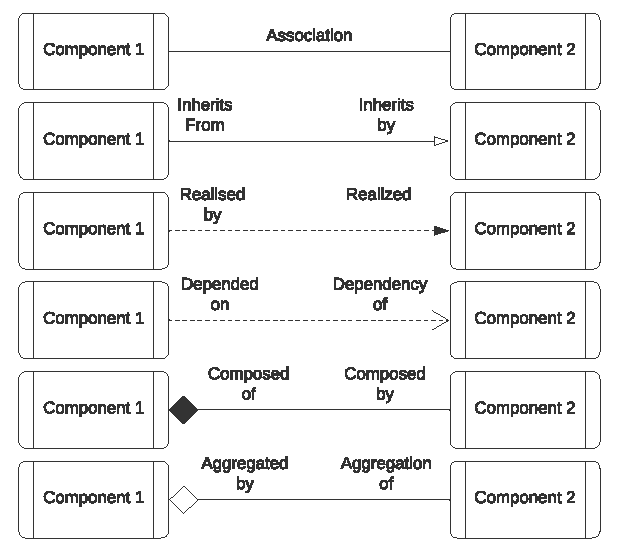
\includegraphics[width=0.5\textwidth]{figures/legenda.pdf}
  \caption[UML Notation used]{UML notation}
  \label{fi:class_diagram_relationship_notation}
\end{figure}
%\include{Appendices/AppendixC}

%----------------------------------------------------------------------------------------
%	BIBLIOGRAPHY
%----------------------------------------------------------------------------------------

\emergencystretch=1em
\printbibliography[heading=bibintoc, keyword=ns, title=Bibliography Normalized Systems]
\printbibliography[heading=bibintoc, keyword=ca, title=Bibliography Clean Architecture]
\printbibliography[heading=bibintoc, keyword=proto, title=Prototype examples,]


%----------------------------------------------------------------------------------------

\end{document}  
